%% contents/sqp.tex
%% Copyright 2021-2022 Tom M. Ragonneau
%
% This work may be distributed and/or modified under the
% conditions of the LaTeX Project Public License, either version 1.3
% of this license or (at your option) any later version.
% The latest version of this license is in
%   http://www.latex-project.org/lppl.txt
% and version 1.3 or later is part of all distributions of LaTeX
% version 2005/12/01 or later.
%
% This work has the LPPL maintenance status `maintained'.
%
% The Current Maintainer of this work is Tom M. Ragonneau.
\chapter{The \glsfmtshort{sqp} method \textemdash\ an overview and some perspectives}
\label{ch:sqp}

This chapter introduces the well-known \gls{sqp} method, assuming that the derivatives of the objective and constraint functions are available.
We first present the general \gls{sqp} framework and some insights into its subproblem from four different angles in \cref{sec:sqp-method}.
\Cref{sec:sqp-merit-functions} then introduces the concept of merit function used in globalization strategies for the \gls{sqp} method.
Further, \cref{sec:sqp-trust-region} focuses on the trust-region \gls{sqp} framework and some composite-step methods for solving its subproblem, referred to as the Byrd-Omojokun, Vardi, and \gls{cdt} approaches.
\Cref{sec:existing-sqp-software} briefly mentions some well-known software based on the \gls{sqp} method.

Most of the materials in this chapter are not new, and can be found for example in~\cite{Boggs_Tolle_1995,Gould_Toint_2000},~\cite[Ch.~15]{Conn_Gould_Toint_2000},~\cite[Ch.~12]{Sun_Yuan_2006},~\cite[Ch.~18]{Nocedal_Wright_2006}, and~\cite{Schittkowski_Yuan_2011,Gill_Wong_2011}.
However, we highlight \cref{thm:sqp-path,thm:auglag-sqp-3,prop:vardi-byrd-omojokun}, which are new to the best of our knowledge, although the last two are easy to establish.
\Cref{thm:sqp-path} interprets the objective function of the \gls{sqp} subproblem as a quadratic approximation of the original objective function in the tangent space of a surface.
This explains in a new way why the \gls{sqp} subproblem should not minimize second-order Taylor expansion of the original objective function unless the constraints are all linear.
\Cref{thm:auglag-sqp-3} shows that the augmented Lagrangian of the \gls{sqp} subproblem is a particular quadratic approximation of the augmented Lagrangian used in~\cite{Niu_Yuan_2010,Wang_Yuan_2014}.
Finally, \cref{prop:vardi-byrd-omojokun} interprets the Vardi approach as an approximation to the Byrd-Omojokun approach.

\section{The method}
\label{sec:sqp-method}

Throughout this chapter, we consider a problem of the form
\begin{subequations}
    \label{eq:problem-cobyqa-sqp}
    \begin{align}
        \min        & \quad \obj(\iter) \label{eq:problem-cobyqa-sqp-obj}\\
        \text{s.t.} & \quad \con{i}(\iter) \le 0, ~ i \in \iub, \label{eq:problem-cobyqa-sqp-ub}\\
                    & \quad \con{i}(\iter) = 0, ~ i \in \ieq, \label{eq:problem-cobyqa-sqp-eq}\\
                    & \quad \iter \in \R^n. \nonumber
    \end{align}
\end{subequations}

Note that the problem~\cref{eq:problem-cobyqa-sqp} is precisely the problem~\cref{eq:problem-introduction} discussed in \cref{ch:introduction}; hence, all the theory mentioned is applicable.
For our later discussion, recall in particular that the Lagrangian of this problem is defined by
\begin{equation*}
    \lag(\iter, \lm) \eqdef \obj(\iter) + \sum_{\mathclap{i \in \iub \cup \ieq}} \lm_i \con{i}(\iter), \quad \text{for~$\iter \in \R^n$ and~$\lm_i \in \R$, with~$i \in \iub \cup \ieq$,}
\end{equation*}
where~$\lm = [\lm_i]_{i \in \iub \cup \ieq}^{\T}$ is the dual variable of the considered problem.

\subsection{Overview of the method}

The \gls{sqp} method is known to be one of the most powerful methods for solving the problem~\cref{eq:problem-cobyqa-sqp} when derivatives of~$\obj$ and~$\con{i}$, with~$i \in \iub \cup \ieq$, are available.
The classical \gls{sqp} framework is presented in \cref{alg:sqp}.

\begin{algorithm}
    \caption{Classical \glsfmtshort{sqp} method}
    \label{alg:sqp}
    \DontPrintSemicolon
    \onehalfspacing
    \KwData{Initial guess~$\iter[0] \in \R^n$ and estimated Lagrange multiplier~$\lm[0] = [\lm[0]_i]_{i \in \iub \cup \ieq}^{\T}$.}
    \For{$k = 0, 1, \dots$}{
        Define~$H^k \approx \nabla_{x, x}^2 \lag(\iter[k], \lm[k])$\;
        Generate a step~$\step[k] \in \R^n$ by solving approximately
        \begin{subequations}
            \label{eq:sqp-subproblem}
            \begin{algomathalign}
                \min        & \quad \nabla \obj(\iter[k])^{\T} \step + \frac{1}{2} \step^{\T} H^k \step \label{eq:sqp-subproblem-obj}\\
                \text{s.t.} & \quad \con{i}(\iter[k]) + \nabla \con{i}(\iter[k])^{\T} \step \le 0, ~ i \in \iub,\\
                            & \quad \con{i}(\iter[k]) + \nabla \con{i}(\iter[k])^{\T} \step = 0, ~ i \in \ieq,\\
                            & \quad \step \in \R^n, \nonumber
            \end{algomathalign}
        \end{subequations}
        Update the iterate~$\iter[k + 1] \gets \iter[k] + \step[k]$\;
        Estimate the Lagrange multiplier~$\lm[k + 1] = [\lm[k + 1]_i]_{i \in \iub \cup \ieq}^{\T}$\;
    }
\end{algorithm}

The earliest reference to such a method appeared in the Ph.D. thesis of \citeauthor{Wilson_1963}~\cite{Wilson_1963}, with~$H^k = \nabla_{x, x}^2 \lag(\iter[k], \lm[k])$.
\Citeauthor{Robinson_1974}~\cite{Robinson_1974} showed the local R-quadratic convergence rate of this method.
Later, \citeauthor{Garcia-Palomares_Mangasarian_1976}~\cite{Garcia-Palomares_1973,Garcia-Palomares_Mangasarian_1976} modified it using a quasi-Newton update for calculating~$H^k$ and established a local R-superlinear convergence rate for such an algorithm.
A similar method was introduced by \citeauthor{Han_1976}~\cite{Han_1976,Han_1977}, but he only approximated~$\nabla_{x, x}^2 \lag(\iter[k], \lm[k])$, while \citeauthor{Garcia-Palomares_Mangasarian_1976} applied quasi-Newton approximations to the whole matrix~$\nabla^2 \lag(\iter[k], \lm[k])$.
In addition, \citeauthor{Han_1976} introduced a line-search strategy to guarantee the global convergence and local Q-superlinear convergence rate, requiring that~$\nabla_{x, x}^2 \lag(\iter[\ast], \lm[\ast])$ is positive definite at the solution~$(\iter[\ast], \lm[\ast])$.
\Citeauthor{Powell_1978a}~\cite{Powell_1978b,Powell_1978a,Powell_1978c} studied the method in the same direction.
In particular, he proposed to apply the damped BFGS quasi-Newton formula~\cite[Eqs.~(5.8),~(5.9), and~(5.10)]{Powell_1978b} to update~$H^k$.
This formula guarantees the positive definiteness of such a matrix, which is beneficial in practice and theory (see the comments towards the end of~\cite[\S~2]{Powell_1978a}).
Moreover, he introduced a practical line-search technique based on a merit function suggested by \citeauthor{Han_1976}~\cite{Han_1976}.
Furthermore, \citeauthor{Powell_1978c} established the global convergence and the local R-superlinear convergence rate for his method without requiring the positive definiteness of~$\nabla_{x, x}^2 \lag(\iter[\ast], \lm[\ast])$ as \citeauthor{Han_1976} did.
Recognizing the contributions of \citeauthor{Wilson_1963}, \Citeauthor{Han_1976}, and \citeauthor{Powell_1978a}, the \gls{sqp} method is also referred to as the Wilson-Han-Powell method~\cite{Schittkowski_1981,Burke_1992}.
See~\cite{Boggs_Tolle_1995} for a more detailed review of the history, theory, and practice of the \gls{sqp} method.

\subsection{A simple example}
\label{subsec:sqp-simple-example}

In \cref{alg:sqp}, it is crucial that~$H^k$ approximates~$\nabla_{x, x}^2 \lag(\iter[k], \lm[k])$.
It may be tempting to set~$H^k \approx \nabla \obj(\iter[k])$, because the objective function of the \gls{sqp} subproblem would then be a local quadratic approximation of~$\obj$ at~$\iter[k]$.
However, such a naive idea does not work, as illustrated by the following~$2$-dimensional example inspired by \citeauthor{Boggs_Tolle_1995}~\cite[\S~2.2]{Boggs_Tolle_1995}.

We consider
\begin{align*}
    \min        & \quad -\iter_1 - \frac{(\iter_2)^2}{4}\\
    \text{s.t.} & \quad \norm{\iter}^2 - 1 = 0,\\
                & \quad \iter \in \R^2,
\end{align*}
whose solution is~$\iter[\ast] = [1, 0]^{\T}$ with the associated Lagrange multiplier~$\lm[\ast] = 1/2$.
Suppose that we have an iterate~$\iter[k] = [t, 0]^{\T}$ with~$t \approx 1$, so it is already close to the solution.
If~$H^k = \nabla^2 \obj(\iter[k])$, then the \gls{sqp} subproblem becomes
\begin{subequations}
    \begin{align}
        \min        & \quad -\step_1 - \frac{(\step_2)^2}{4} \label{eq:boggs-tolle-sp-obj}\\
        \text{s.t.} & \quad \step_1 = \frac{1 - t^2}{2 t}, \label{eq:boggs-tolle-sp-eq}\\
                    & \quad \step \in \R^2. \nonumber
    \end{align}
\end{subequations}
This subproblem is unbounded from below, regardless of the value of~$t$.
In addition, the more~$\step[k]$ reduces~\cref{eq:boggs-tolle-sp-obj}, the larger~$\norm{\iter[k] + \step[k] - \iter[\ast]}$ is.
If~$t = 1$, we have~$\iter[k] = \iter[\ast]$, but any feasible point~$\step[k]$ for~\cref{eq:boggs-tolle-sp-eq} will push~$\iter[k] + \step[k]$ away from~$\iter[\ast]$, unless~$\step[k]$ is the global maximizer of~\cref{eq:boggs-tolle-sp-obj} subject to~\cref{eq:boggs-tolle-sp-eq}.

Let us now consider the \gls{sqp} subproblem~\cref{eq:sqp-subproblem} with~$H^k = \nabla_{x, x}^2 \lag(\iter[k], \lm[k])$ for a dual variable~$\lm[k] \approx \lm[\ast] = 1/2$.
It is
\begin{align*}
    \min        & \quad -\step_1 + \lm[k] (\step_1)^2 + \bigg( \lm[k] - \frac{1}{4} \bigg) (\step_2)^2\\
    \text{s.t.} & \quad \step_1 = \frac{1 - t^2}{2 t},\\
                & \quad \step \in \R^2. \nonumber
\end{align*}
When~$\lm[k] > 1/4$, the solution to this subproblem is
\begin{equation*}
    \step[k] =
    \begin{bmatrix}
        \dfrac{1 - t^2}{2 t}    & 0
    \end{bmatrix}^{\T}.
\end{equation*}
We thus have
\begin{equation*}
    \iter[k] + \step[k] = 
    \begin{bmatrix}
        \dfrac{t^2 + 1}{2 t}  & 0
    \end{bmatrix}^{\T}.
\end{equation*}
If we set~$\iter[k + 1] = \iter[k] + \step[k]$ and continue to iterate in this way, we will obtain a sequence of iterates that converges quadratically to~$\iter[\ast]$, because
\begin{equation*}
    \norm{\iter[k] + \step[k] - \iter[\ast]} = \frac{(1 - t)^2}{2 \abs{t}} = \bigo(\norm{\iter[k] - \iter[\ast]}^2).
\end{equation*}
This is not surprising, since \citeauthor{Robinson_1974}~\cite{Robinson_1974} showed the local R-quadratic convergence rate of the \gls{sqp} method when~$H^k$ is the exact Hessian matrix of the Lagrangian with respect to~$\iter$.

To summarize, as indicated by this example, choosing~$H^k \approx \nabla_{x, x}^2 \lag(\iter[k], \lm[k])$ instead of~$H^k \approx \nabla \obj(\iter[k])$ in~\cref{eq:sqp-subproblem} is crucial.

\subsection{Interpretations of the \glsfmtshort{sqp} subproblem}
\label{subsec:sqp-interpretation}

To get some insight into the origin of the \gls{sqp} method, we interpret the \gls{sqp} subproblem~\cref{eq:sqp-subproblem}.
In what follows, we focus on only one iteration of \cref{alg:sqp} and hence,~$k$ is fixed.
We will explain why it is reasonable to update~$\iter[k]$ by a solution to~\cref{eq:sqp-subproblem}.

\subsubsection{Bilinear approximation of the \glsfmtlong{kkt} conditions}

This is the most classical interpretation of the \gls{sqp} subproblem.
According to \cref{thm:first-order-necessary-conditions}, if~$\iter[\ast] \in \R^n$ is a local solution to the problem~\cref{eq:problem-cobyqa-sqp}, under some mild assumptions, there exists a Lagrange multiplier~$\lm[\ast] = [\lm[\ast]_i]_{i \in \iub \cup \ieq}^{\T}$ with~$\lm[\ast]_i \in \R$ for all~$i \in \iub \cup \ieq$ such that
\begin{subequations}
    \label{eq:sqp-kkt}
    \begin{empheq}[left=\empheqlbrace]{alignat=1}
        & \nabla_x \lag(\iter[\ast], \lm[\ast]) = 0,\\
        & \con{i}(\iter[\ast]) \le 0, ~ i \in \iub,\\
        & \con{i}(\iter[\ast]) = 0, ~ i \in \ieq,\\
        & \lm[\ast]_i \con{i}(\iter[\ast]) = 0, ~ i \in \iub, \label{eq:sqp-kkt-complementary-slackness}\\
        & \lm[\ast]_i \ge 0, ~ i \in \iub.
    \end{empheq}
\end{subequations}
Regard~\cref{eq:sqp-kkt} as a nonlinear system of inequalities and equalities, and~$(\iter[k], \lm[k])$ as an approximation of~$(\iter[\ast], \lm[\ast])$.
If we want to solve this system by the Newton-Raphson method\footnote{Discussions are needed on how to apply the Newton-Raphson method to systems of nonlinear inequalities and equalities. We will not go further in this direction but refer to \cite{Pshenichnyi_1970a,Pshenichnyi_1970b,Robinson_1972b,Daniel_1973} for fundamental works on this topic.} starting from~$(\iter[k], \lm[k])$, we would seek a step~$(\step, \mu)$ that satisfies the system
\begin{subequations}
    \label{eq:sqp-kkt-linearization}
    \begin{empheq}[left=\empheqlbrace]{alignat=1}
        & \nabla_x \lag(\iter[k], \lm[k] + \mu) + \nabla_{x, x}^2 \lag(\iter[k], \lm[k]) \step = 0,\\
        & \con{i}(\iter[k]) + \nabla \con{i}(\iter[k])^{\T} \step \le 0, ~ i \in \iub,\\
        & \con{i}(\iter[k]) + \nabla \con{i}(\iter[k])^{\T} \step = 0, ~ i \in \ieq,\\
        & \lm[k]_i [\con{i}(\iter[k]) + \nabla \con{i}(\iter[k])^{\T} \step] + \mu_i \con{i}(\iter[k]) = 0, ~ i \in \iub, \label{eq:sqp-kkt-linearization-complementary-slackness}\\
        & \lm[k]_i + \mu_i \ge 0, ~ i \in \iub,
    \end{empheq}
\end{subequations}
which is a linear approximation of~\cref{eq:sqp-kkt} at~$(\iter[k], \lm[k])$.
However, as pointed out by \citeauthor{Robinson_1972a}~\cite[Rem.~3]{Robinson_1972a}, an objection to such a method is that it would not solve even a linear program in one iteration.
To cope with this deffect, we let~$(d, \mu)$ solve instead the following bilinear approximation of~\cref{eq:sqp-kkt},
\begin{subequations}
    \label{eq:sqp-subproblem-kkt}
    \begin{empheq}[left=\empheqlbrace]{alignat=1}
        & \nabla_x \lag(\iter[k], \lm[k] + \mu) + \nabla_{x, x}^2 \lag(\iter[k], \lm[k]) \step = 0,\\
        & \con{i}(\iter[k]) + \nabla \con{i}(\iter[k])^{\T} \step \le 0, ~ i \in \iub,\\
        & \con{i}(\iter[k]) + \nabla \con{i}(\iter[k])^{\T} \step = 0, ~ i \in \ieq,\\
        & (\lm[k]_i + \mu_i) [\con{i}(\iter[k]) + \nabla \con{i}(\iter[k])^{\T} \step] = 0, ~ i \in \iub, \label{eq:sqp-subproblem-kkt-complementary-slackness}\\
        & \lm[k]_i + \mu_i \ge 0, ~ i \in \iub.
    \end{empheq}
\end{subequations}
Its only difference with the system~\cref{eq:sqp-kkt-linearization} lies in the condition~\cref{eq:sqp-subproblem-kkt-complementary-slackness}, which includes the bilinear term~$\mu_i \nabla \con{i}(\iter[k])^{\T} \step$.
If the problem~\cref{eq:problem-cobyqa-sqp} is a linear program, then~\cref{eq:sqp-subproblem-kkt} is precisely its \gls{kkt} system, while~\cref{eq:sqp-kkt-linearization} is only an approximation.
Observe that the bilinear system~\cref{eq:sqp-subproblem-kkt} is nothing but the \gls{kkt} conditions of the \gls{sqp} subproblem~\cref{eq:sqp-subproblem}, with~$\lm[k] + \mu$ being the Lagrange multiplier.
Therefore, a \gls{kkt} pair for the \gls{sqp} subproblem~\cref{eq:sqp-subproblem} is similar to a Newton-Raphson step for the \gls{kkt} system of the problem~\cref{eq:problem-cobyqa-sqp}, and it is even better in the sense that the resulting method solves a linear program in one iteration.

Note that discrepancy between the systems~\cref{eq:sqp-kkt-linearization,eq:sqp-subproblem-kkt} disappears if~$\iub = \emptyset$ in the problem~\cref{eq:problem-cobyqa-sqp} and hence, a \gls{kkt} pair for the \gls{sqp} subproblem~\cref{eq:sqp-subproblem} is exactly a Newton-Raphson step for the \gls{kkt} system of the problem~\cref{eq:problem-cobyqa-sqp} in such a situation.

\subsubsection{Approximation of a modified Lagrangian}

This interpretation is due to \citeauthor{Robinson_1972a}~\cite[Rem.~4]{Robinson_1972a}.
Let~$\widetilde{\lag}$ be the function
\begin{equation*}
    \widetilde{\lag}(\iter, \lm) \eqdef \obj(\iter) + \sum_{\mathclap{i \in \iub \cup \ieq}} \lm_i \delta_i(\iter), \quad \text{for~$\iter \in \R^n$ and~$\lm_i \in \R$, with~$i \in \iub \cup \ieq$},
\end{equation*}
where~$\delta_i$, for~$i \in \iub \cup \ieq$, is defined by
\begin{equation*}
    \delta_i(\iter) \eqdef \con{i}(\iter) - \con{i}(\iter[k]) - \nabla \con{i}(\iter[k])^{\T} (\iter - \iter[k]), \quad \text{for~$\iter \in \R^n$.}
\end{equation*}
The function~$\delta_i$ is referred to as the departure from linearity\footnote{When~$\con{i}$ is strictly convex,~$\delta_i$ defines the Bregman distance~\cite{Bregman_1967} associated with~$\con{i}$.} for~$\con{i}$ at the point~$\iter[k]$ (see~\cite[\S~2]{Gill_Wong_2011} and~\cite[\S~2.3]{Gill_Murray_Saunders_2005}).
The \gls{sqp} subproblem~\cref{eq:sqp-subproblem} with~$H^k = \nabla_{x, x}^2 \lag(\iter[k], \lm[k])$ can then be seen as the minimization of the second-order Taylor approximation of~$\widetilde{\lag}$ subject to the linearizations of the constraints~\cref{eq:problem-cobyqa-sqp-ub,eq:problem-cobyqa-sqp-eq} at~$(\iter[k], \lm[k])$, i.e.,
\begin{align*}
    \min        & \quad \nabla_x \widetilde{\lag}(\iter[k], \lm[k])^{\T} \step + \frac{1}{2} \step^{\T} \nabla_{x, x}^2 \widetilde{\lag}(\iter[k], \lm[k]) \step\\
    \text{s.t.} & \quad \con{i}(\iter[k]) + \nabla \con{i}(\iter[k])^{\T} \step \le 0, ~ i \in \iub,\\
                & \quad \con{i}(\iter[k]) + \nabla \con{i}(\iter[k])^{\T} \step = 0, ~ i \in \ieq,\\
                & \quad \step \in \R^n.
\end{align*}

By expressing its subproblem in this form, we see that the \gls{sqp} method is a special case of \citeauthor{Robinson_1972a}'s method~\cite{Robinson_1972a}, known to have a local R-quadratic convergence rate.

\subsubsection{Approximation of the objective function in the tangent space of a surface}

% Inspired by an observation in~\cite[\S~2]{Gill_Wong_2011}, we can also interpret the \gls{sqp} subproblem as minimizing an approximation of the objective function in the tangent space of the feasible set.
Inspired by an observation in~\cite[\S~2]{Gill_Wong_2011}, we can also interpret the objective function of the \gls{sqp} subproblem as an approximation of the original objective function in the tangent space of a particular surface described below.
As shown in \cref{thm:sqp-path}, when approximating~$\obj$ in this space, we will naturally get the Hessian matrix of the Lagrangian in the second-order term.

For this interpretation, we focus on the equality-constrained problem
\begin{subequations}
    \label{eq:problem-cobyqa-auglag}
    \begin{align}
        \min        & \quad \obj(\iter)\\
        \text{s.t.} & \quad h(\iter) = 0,\\
                    & \quad \iter \in \R^n, \nonumber
    \end{align}
\end{subequations}
with~$h : \R^n \to \R^m$.
Recall that the Lagrangian function of~\cref{eq:problem-cobyqa-auglag} is
\begin{equation*}
    \lag(\iter, \lm) \eqdef \obj(\iter) + \lm^{\T} h(\iter), \quad \text{for~$\iter \in \R^n$ and~$\lm \in \R^m$.}
\end{equation*}

Let~$\bar{\iter} \in \R^n$,~$\bar{\lm} \in \R^m$ be given, and define
\begin{equation*}
    Q(\step) \eqdef \obj(\bar{\iter}) + \nabla \obj(\bar{\iter})^{\T} \step + \frac{1}{2} \step^{\T} \nabla_{x, x}^2 \lag(\bar{\iter}, \bar{\lm}) \step.
\end{equation*}
If~$\bar{\iter}$ and~$\bar{\lm}$ represent the current iterate and approximate Lagrange multiplier, then~$Q$ is the objective function of the \gls{sqp} subproblem with an exact second-order term.
% Therefore, the \gls{sqp} subproblem approximates~$\obj$ by~$Q$ and the feasible set by its tangent space.
% Such an approximation is reasonable only if~$Q$ approximates~$\obj$ in this tangent space, which turns out to be true, as detailed by \cref{thm:sqp-path}.
% Such an approximation is reasonable only if~$Q$ approximates~$\obj$ in this tangent space.
At first glance,~$Q$ does not seem to be a natural approximation of~$\obj$ due to its second-order term.
However, this approximation turns out to be indeed natural if we focus on the contour surface of~$h$ at~$\bar{\iter}$ and its tangent space.
This is detailed in \cref{thm:sqp-path}.

\begin{theorem}
    \label{thm:sqp-path}
    Assume that~$\obj$ and~$h$ are twice differentiable with~$\nabla^2 \obj$ being locally Lipschitz continuous.
    % Suppose that~$\bar{\iter}$ is feasible for~\cref{eq:problem-cobyqa-auglag}.
    Consider a curve parametrized by~$\iter : \R \to \R^n$, satisfying
    \begin{equation}
        \label{eq:sqp-path}
        h(\iter(t)) = h(\bar{\iter}) \quad \text{for all~$t \in \R$}, \quad \text{and} \quad \iter(0) = \bar{\iter}.
    \end{equation}
    If~$\iter$ is twice differentiable and~$\iter''$ is locally Lipschitz continuous, then there exist constants~$\nu \ge 0$ and~$\epsilon > 0$ such that
    \begin{equation*}
        \abs{\obj(\iter(t)) - Q(x'(0) t)} \le \bigg( \nu t + \frac{1}{2}\abs{\iter''(0)^{\T} [\nabla \obj(\bar{\iter}) + \nabla h(\bar{\iter})^{\T} \bar{\lm}]} \bigg) t^2 \quad \text{for all~$t \in (-\epsilon, \epsilon)$.}
    \end{equation*}
\end{theorem}

\begin{proof}
    Define
    \begin{equation*}
        \phi(t) \eqdef \obj(x(t)), \quad \text{for~$t \in \R$.}
    \end{equation*}
    By assumption,~$\phi$ is twice differentiable and there exists~$\epsilon > 0$ such that~$\phi''$ is Lipschitz continuous in~$(-\epsilon, \epsilon)$.
    Let~$\widehat{\phi}$ be the second-order Taylor expansion of~$\phi$ at~$0$.
    Then
    \begin{equation}
        \label{eq:sqp-path-proof-2}
        \abs{\obj(\iter(t)) - Q(\iter'(0) t)} \le \abs{\phi(t) - \widehat{\phi}(t)} + \abs{\widehat{\phi}(t) - Q(\iter'(0) t)},
    \end{equation}
    and the Lipschitz continuity of~$\phi''$ ensures the existence of a constant~$\nu \ge 0$ such that
    \begin{equation}
        \label{eq:sqp-path-proof-3}
        \abs{\phi(t) - \widehat{\phi}(t)} \le \nu t^3 \quad \text{for~$t \in (-\epsilon, \epsilon)$.}
    \end{equation}
    We now bound~$\abs{\widehat{\phi}(t) - Q(\iter'(0) t)}$.
    Noting that~$\iter(0) = \bar{\iter}$, we have
    \begin{subequations}
        \label{eq:sqp-path-proof-1}
        \begin{empheq}[left=\empheqlbrace]{alignat=1}
            & \phi'(0) = \iter'(0)^{\T} \nabla \obj(\bar{\iter}),\\
            & \phi''(0) = \iter'(0)^{\T} \nabla^2 \obj(\bar{\iter}) \iter'(0) + \iter''(0)^{\T} \nabla \obj(\bar{\iter}). \label{eq:sqp-path-proof-1-2}
        \end{empheq}
    \end{subequations}
    According to~\cref{eq:sqp-path-proof-1}, only the second-order terms of~$\widehat{\phi}(t)$ and~$Q(\iter'(0) t)$ differ. Hence,
    \begin{subequations}
        \label{eq:sqp-path-proof-4}
        \begin{align}
            \abs{\widehat{\phi}(t) - Q(x'(0) t)}    & = \frac{t^2}{2} \abs{\phi''(0) - \iter'(0)^{\T} \nabla_{x, x}^2 \lag(\bar{\iter}, \bar{\lm}) \iter'(0)}\\
                                                    & = \frac{t^2}{2} \abs[\bigg]{\iter''(0)^{\T} \nabla \obj(\bar{\iter}) - \sum_{i = 1}^m \bar{\lm}_i \iter'(0) \nabla^2 h_i(\bar{\iter}) \iter'(0)}, \label{eq:sqp-path-proof-4-2}
        \end{align}
    \end{subequations}
    where the second equality uses the formula of~$\phi''(0)$ in~\cref{eq:sqp-path-proof-1-2} and the definition of~$\lag$.
    Moreover, since~$h(\iter(t)) = h(\bar{\iter})$ for all~$t \in \R$, we have
    \begin{equation*}
        0 = \frac{\du^2}{\du t^2} h_i(\iter(t)) \bigg\vert_{t = 0} = \iter'(0)^{\T} \nabla^2 h_i(\bar{\iter}) \iter'(0) + \iter''(0)^{\T} \nabla h_i(\bar{\iter}), \quad \text{for~$i \in \set{1, 2, \dots, m}$.}
    \end{equation*}
    Therefore,~$\iter'(0)^{\T} \nabla^2 h_i(\bar{\iter}) \iter'(0) = -\iter''(0)^{\T} \nabla h_i(\bar{\iter})$ for each~$i$ and hence,~\cref{eq:sqp-path-proof-4} leads to
    \begin{equation}
        \label{eq:sqp-path-proof-5}
        \abs{\widehat{\phi}(t) - Q(x'(0) t)} \le \frac{t^2}{2} \abs{\iter''(0)^{\T} [\nabla \obj(\bar{\iter}) + \nabla h(\bar{\iter})^{\T} \bar{\lm}]}.
    \end{equation}
    Plugging~\cref{eq:sqp-path-proof-3,eq:sqp-path-proof-5} into~\cref{eq:sqp-path-proof-2}, we obtain the desired result.
\end{proof}

Note that~$\iter'(0)$ in \cref{thm:sqp-path} is a vector in
\begin{equation*}
    \mathcal{T}_{\bar{\iter}} = \set{\step \in \R^n : \nabla h(\bar{\iter}) \step = 0}.
\end{equation*}
This is the tangent space of
\begin{equation*}
    \mathcal{S}_{\bar{x}} = \set{\iter \in \R^n : h(\iter) = h(\bar{\iter})},
\end{equation*}
at~$\bar{\iter}$, and~$\mathcal{S}_{\bar{x}}$ is the contour surface of the constraints at~$\bar{\iter}$.
Therefore, \cref{thm:sqp-path} reveals that the objective function of the \gls{sqp} subproblem is a quadratic approximation of~$\obj$ in this tangent space.

However, the feasible region of the \gls{sqp} subproblem is in general not the tangent
space~$\mathcal{T}_{\bar{\iter}}$ but the linearized feasible direction set
\begin{equation*}
    \mathcal{F}_{\bar{\iter}}^{\mathsf{L}} = \set{\step \in \R^n : h(\bar{\iter}) +\nabla h(\bar{\iter}) \step  = 0},
\end{equation*}
which is assumed nonempty for the current discussion.
This set equals~$\mathcal{T}_{\bar{\iter}}$ only if~$\bar{\iter}$ is feasible so that~$h(\bar{\iter}) = 0$.
When~$\bar{\iter}$ is infeasible, $\mathcal{F}_{\bar{\iter}}^{\mathsf{L}}$ is a shifted copy of~$\mathcal{T}_{\bar{\iter}}$ as illustrated in \cref{fig:sqp-path}.
The distance between~$\mathcal{F}_{\bar{\iter}}^{\mathsf{L}}$ and~$\mathcal{T}_{\bar{\iter}}$ is~$\delta_{\bar{\iter}} = \norm{\step[\ast]} = \norm{\nabla h(\bar{\iter})^{\dagger} h(\bar{\iter})}$, where~$\step[\ast]$ is the projection of~$0 \in \mathcal{T}_{\bar{\iter}}$ onto~$\mathcal{F}_{\bar{\iter}}^{\mathsf{L}}$, and~$\nabla h(\bar{\iter})^{\dagger}$ denotes the Moore-Penrose pseudoinverse of~$\nabla h(\bar{\iter})$.
The purpose of this shifting is to improve the feasibility.
% Indeed, if~$h$ is twice continuously differentiable, then its Taylor expansion provides~$\norm{h(\bar{\iter} + \step)} =\bigo(\norm{\step}^2)$ for all $\step$ in a bounded subset of~$\mathcal{F}_{\bar{\iter}}^{\mathsf{L}}$, whereas~$\norm{h(\bar{\iter} + \step)} = \norm{h(\bar{\iter})} + \bigo(\norm{\step}^2)$ if~$\step$ stays in a bounded subset of~$\mathcal{T}_{\bar{\iter}}$.
Indeed, if~$h$ is twice continuously differentiable, then its Taylor expansion provides~$\norm{h(\bar{\iter} + \step)} = \bigo(\norm{\step}^2)$ for all~$\step$ in a bounded subset of~$\mathcal{F}_{\bar{\iter}}^{\mathsf{L}}$, which further implies~$\norm{h(\bar{\iter} + \step)} = \bigo(\norm{h(\bar{\iter})}^2)$ unless~$\norm{\step}$ is much larger than~$\norm{\step[\ast]}$; in contrast,~$\norm{h(\bar{\iter} + \step)} = \norm{h(\bar{\iter})} + \bigo(\norm{\step}^2)$ if~$\step$ stays in a bounded subset of~$\mathcal{T}_{\bar{\iter}}$.

\begin{figure}[ht]
    \centering
    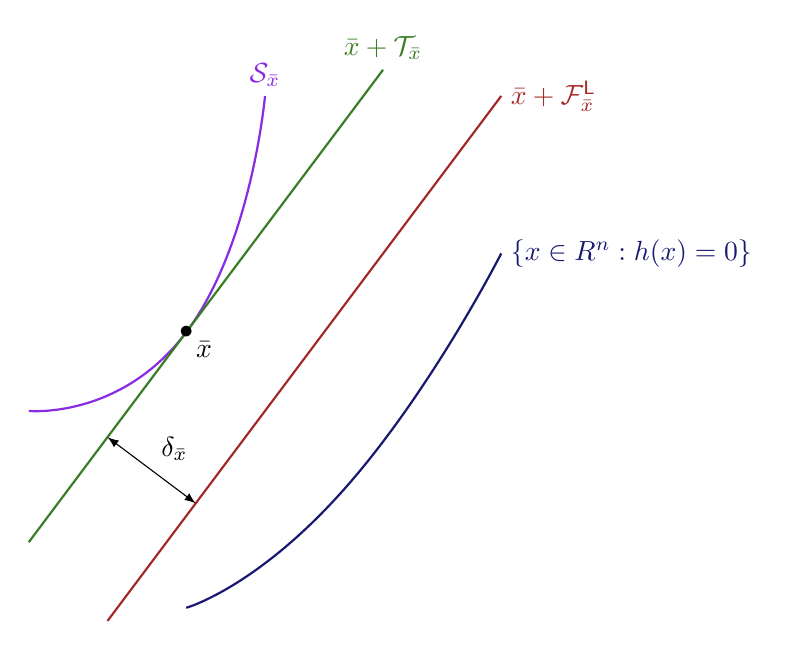
\begin{tikzpicture}
        \draw[thick,BlueViolet] plot[smooth,tension=1] coordinates {(0,2) (2,3) (3,6)};
        \draw[thick,MidnightBlue] plot[smooth,tension=1] coordinates {(2,-0.5) (4,1) (6,4)};
        \draw[thick,OliveGreen] (0,1/3) -- (4.5,19/3);
        \draw[thick,Brown] (1,-2/3) -- (6,18/3);
        \draw[latex-latex] (1,5/3) -- (53/25,62/75);
        
        \node at (2,3) {$\bullet$};
        
        \node[below right] at (2,3) {$\bar{x}$};
        \node[above right] at (39/25,187/150) {$\delta_{\bar{x}}$};
        \node[above,BlueViolet] at (3,6) {$\mathcal{S}_{\bar{x}}$};
        \node[above,OliveGreen] at (4.5,19/3) {$\bar{x} + \mathcal{T}_{\bar{x}}$};
        \node[right,Brown] at (6,18/3) {$\bar{x} + \mathcal{F}_{\bar{x}}^{\mathsf{L}}$};
        \node[right,MidnightBlue] at (6,4) {$\{x \in \mathbb{R}^n : h(x) = 0\}$};
    \end{tikzpicture}
    \caption{An illustration of~$\mathcal{T}_{\bar{\iter}}$,~$\mathcal{S}_{\bar{x}}$,~$\mathcal{F}_{\bar{\iter}}^{\mathsf{L}}$, and the feasible set}
    \label{fig:sqp-path}
\end{figure}

Therefore, the \gls{sqp} subproblem models the objective function in the tangent space of the contour surface of the constraint at the current iterate, and then minimizes this model in a linear space that shifts the tangent space towards improvement of feasibility.
% Thanks to the~$\nabla_{x, x}^2 \lag(\bar{\iter}, \bar{\lm})$ term, the model enjoys a second to third order accuracy if $(\bar{\iter}, \bar{\lm})$ is a good approximate \gls{kkt} pair.
% If we replace~$\nabla_{x, x}^2 \lag(\bar{\iter}, \bar{\lm})$ with~$\nabla^2 \obj(\bar{\iter})$, the accuracy is only second order.
We observe that the magnitude of~$\nabla \obj(\bar{\iter}) + \nabla h(\bar{\iter})^{\T} \bar{\lm}$ affects the quality of the model in general, as indicated by the error estimation in \cref{thm:sqp-path}.
If~$(\bar{\iter}, \bar{\lm})$ is close to a \gls{kkt} pair, then~$\norm{\nabla \obj(\bar{\iter}) + \nabla h(\bar{\iter})^{\T} \bar{\lm}}$ is small.
On the other hand, if we defined~$\nabla^2 Q$ by~$\nabla^2 \obj(\bar{x})$ instead of~$\nabla_{x, x}^2 \lag(\bar{\iter}, \bar{\lm})$, then under the assumptions of \cref{thm:sqp-path}, we would have
\begin{equation*}
    \abs{\obj(\iter(t)) - Q(x'(0) t)} \le \bigg( \nu t + \frac{1}{2}\abs{\iter''(0)^{\T} \nabla \obj(\bar{\iter})} \bigg) t^2 \quad \text{for all~$t \in (-\epsilon, \epsilon)$,}
\end{equation*}
which can be obtained by setting~$\bar{\lm} = 0$ in \cref{thm:sqp-path}.
However, since we are considering constrained optimization, we cannot expect~$\norm{\nabla \obj(\bar{\iter})}$ to be small even if~$\bar{\iter}$ is close to a solution unless no constraint is active at this solution.
This explains why the second-order term of the \gls{sqp} subproblem should be defined by the Hessian matrix of the Lagrangian, rather than that of~$\obj$.

More geometrically speaking, when we regard~$\obj$ as a function on the surface~$\mathcal{S}_{\bar{\iter}}$ and approximate it in the tangent space~$\mathcal{T}_{\bar{\iter}}$, the second-order Taylor expansion of~$\obj$ does not attain the same accuracy as it does in~$\R^n$, because neither this Taylor expansion nor~$\mathcal{T}_{\bar{\iter}}$ can reflect the curvature information
of~$\mathcal{S}_{\bar{\iter}}$.
In contrast, the objective function of the \gls{sqp} subproblem achieves a better accuracy by including such curvature information via~$\nabla_{x, x}^2 \lag(\bar{\iter}, \bar{\lm})$.

It is worth mentioning that \cref{thm:sqp-path} still holds if~$\iter$ satisfies
\begin{equation}
    \label{eq:sqp-path-alt}
    \bar{\lm}^{\T} h(\iter(t)) = \bar{\lm}^{\T} h(\bar{\iter}) \quad \text{for all~$t \in \R$}, \quad \text{and} \quad \iter(0) = \bar{\iter}
\end{equation}
instead of~\cref{eq:sqp-path}.
Given~\cref{eq:sqp-path-alt}, we will have
\begin{equation*}
    0 = \frac{\du^2}{\du t^2} \bar{\lm}^{\T} h(\iter(t)) \bigg\vert_{t = 0} = \bar{\lm}^{\T} \nabla h(\bar{\iter}) \iter''(0) + \sum_{i = 1}^n \bar{\lm}_i \iter'(0)^{\T} \nabla^2 h_i(\bar{\iter}) \iter'(0).
\end{equation*}
Plugging this into~\cref{eq:sqp-path-proof-4-2}, we obtain again~\cref{eq:sqp-path-proof-5} and hence, establish the same estimation of~$\abs{\obj(\iter(t)) - Q(x'(0) t)}$.
Therefore, $Q$ is indeed a quadratic approximation of~$\obj$ in
\begin{equation*}
    \mathcal{T}_{\bar{\iter}, \bar{\lm}} = \set{\step \in \R^n : \bar{\lm}^{\T} \nabla h(\bar{\iter}) \step = 0},
\end{equation*}
which is linear space that contains~$\mathcal{T}_{\bar{\iter}}$ as a subset. 
Note that the dimension of~$\mathcal{T}_{\bar{\iter}, \bar{\lm}}$ is at least~$n - 1$, while that of~$\mathcal{T}_{\bar{\iter}}$ is~$n - \rank(\nabla h(\bar{\iter}))$.

\subsection{Lagrangian and augmented Lagrangian of the \glsfmtshort{sqp} subproblem}
\label{subsec:lagrangian-augmented-lagrangian}

In this section, we study the Lagrangian and the augmented Lagrangian of the \gls{sqp} subproblem and observe their relations with those of the original optimization problem.
We also point out that the augmented Lagrangian of the \gls{sqp} subproblem is exactly the approximate augmented Lagrangian used in~\cite{Niu_Yuan_2010,Wang_Yuan_2014}.

For simplicity, instead of the problem~\cref{eq:problem-cobyqa-sqp}, we consider still the problem~\cref{eq:problem-cobyqa-auglag}.
Let~$\iter[k] \ge 0$ and~$\lm[k] \in \R^m$ be given.
Correspondingly, the \gls{sqp} subproblem of the problem~\cref{eq:problem-cobyqa-auglag} is
\begin{subequations}
    \label{eq:sqp-subproblem-auglag}
    \begin{align}
        \min        & \quad \obj(\iter[k]) + \nabla \obj(\iter[k])^{\T} \step + \frac{1}{2} \step^{\T} H^k \step \label{eq:sqp-subproblem-auglag-obj}\\
        \text{s.t.} & \quad h(\iter[k]) + \nabla h(\iter[k]) \step = 0,\\
                    & \quad \iter[k] + \step \ge 0, ~ \step \in \R^n,
    \end{align}
\end{subequations}
with~$H^k \approx \nabla_{x, x}^2 \lag(\iter[k], \lm[k])$.
Note that the constant term~$\obj(\iter[k])$ in~\cref{eq:sqp-subproblem-auglag-obj} may be excluded, as in~\cref{eq:sqp-subproblem-obj}, but including it facilitates the discussion in the sequel.

Recall that the augmented Lagrangian~\cite{Hestenes_1969,Powell_1969,Rockafellar_1973} of the problem~\cref{eq:problem-cobyqa-auglag} is
\begin{equation}
    \label{eq:augmented-lagrangian-inequality}
    \auglag(\iter, \lm) \eqdef \lag(\iter, \lm) + \frac{\gamma}{2} \norm{h(\iter)}^2, \quad \text{for~$\iter \ge 0$ and~$\lm \in \R^m$,}
\end{equation}
\nomenclature[Fd]{$\auglag$}{Augmented Lagrangian function}%
where~$\gamma \ge 0$ is a penalty parameter.
Denote by~$\lagalt$ the Lagrangian of the \gls{sqp} subproblem~\cref{eq:sqp-subproblem-auglag}, i.e.,
\begin{align*}
    \lagalt(\step, \lm) & \eqdef \obj(\iter[k]) + \nabla \obj(\iter[k])^{\T} \step + \frac{1}{2} \step^{\T} H^k \step\\
                        & \qquad + \lm^{\T} [h(\iter[k]) + \nabla h(\iter[k]) \step], \quad \text{for~$\step \ge -\iter[k]$ and~$\lm \in \R^m$,}
\end{align*}
and by~$\auglagalt$ the augmented Lagrangian of the \gls{sqp} subproblem~\cref{eq:sqp-subproblem-auglag}, i.e.,
\begin{equation*}
    \auglagalt(\step, \lm) \eqdef \lagalt(\step, \lm) + \frac{\gamma}{2} \norm{h(\iter[k]) + \nabla h(\iter[k]) \step}^2, \quad \text{for~$\step \ge -\iter[k]$ and~$\lm \in \R^m$.}
\end{equation*}

We now present some relations between~$\lag$ and~$\lagalt$, and between~$\auglag$ and~$\auglagalt$.

\begin{theorem}
    \label{thm:auglag-sqp-1}
    Assume that~$\obj$ and~$h$ are twice differentiable.
    If~$H^k = \nabla_{x, x}^2 \lag(\iter[k], \lm[k])$, then~$\lagalt(\step, \lm[k])$ is the second-order Taylor expansion of~$\lag(\iter[k] + \step, \lm[k])$ with respect to~$d$ at~$0$.
\end{theorem}

\begin{proof}
    This theorem can be verified by a straightforward calculation.
\end{proof}

\begin{theorem}
    \label{thm:auglag-sqp-2}
    Assume that~$\obj$ and~$h$ are twice differentiable.
    If
    \begin{equation}
        \label{eq:auglag-sqp-2}
        H^k = \nabla^2 \obj(\iter[k]) + \sum_{i = 1}^m [\lm[k]_i + \gamma h_i(\iter[k])] \nabla^2 h_i(\iter[k]),
    \end{equation}
    then~$\auglagalt(\step, \lm[k])$ is the second-order Taylor expansion of~$\auglag(\iter[k] + d, \lm[k])$ with respect to~$d$ at~$0$.
\end{theorem}

\begin{proof}
    By direct calculations, we have
    \begin{equation*}
        \nabla_x \auglag(\iter[k], \lm[k]) = \nabla_x \lag(\iter[k], \lm[k]) + \gamma \nabla h(\iter[k])^{\T} h(\iter[k]),
    \end{equation*}
    and
    \begin{equation*}
        \nabla_{x, x}^2 \auglag(\iter[k], \lm[k]) = \nabla_{x, x}^2 \lag(\iter[k], \lm[k]) + \gamma \bigg[ \nabla h(\iter[k])^{\T} \nabla h(\iter[k]) + \sum_{i = 1}^m h_i(\iter[k]) \nabla^2 h_i(\iter[k]) \bigg].
    \end{equation*}
    Therefore, the second-order Taylor expansion of~$\auglag(\iter[k] + d, \lm[k])$ with respect to~$d$ at~$0$ is
    \begin{equation*}
        \auglag(\iter[k] + d, \lm[k]) = \lag(\iter[k], \lm[k]) + \nabla_x \lag(\iter[k], \lm[k])^{\T} d + \frac{1}{2} d^{\T} H^k d + \frac{\gamma}{2} \norm{h(\iter[k]) + \nabla h(\iter[k]) d}^2 + \smallo(\norm{d}^2),
    \end{equation*}
    \nomenclature[Nh]{$\smallo(\cdot)$}{Little-O notation}%
    where~$H^k$ is defined by~\cref{eq:auglag-sqp-2}.
\end{proof}

Intriguingly, an augmented Lagrangian method for solving the problem~\cref{eq:problem-cobyqa-auglag} updates traditionally the dual variable~$\lm[k]$ by
\begin{equation*}
    \lm[k + 1] = \lm[k] + \gamma h(\iter[k]).
\end{equation*}
Therefore, the second-order Taylor expansion of~$\auglag$ can be interpreted as the augmented Lagrangian of the \gls{sqp} subproblem~\cref{eq:sqp-subproblem-auglag} with~$H^k = \nabla_{x, x}^2 \lag(\iter[k], \lm[k + 1])$.

There is an interesting connection between the augmented Lagrangian of the \gls{sqp} subproblem~\cref{eq:sqp-subproblem-auglag} and the trust-region augmented Lagrange methods studied in~\cite{Niu_Yuan_2010,Wang_Yuan_2014}.
These methods employ the approximation
\begin{equation}
    \label{eq:niu-yuan-auglag}
    \auglag(\iter[k] + \step, \lm[k]) \approx \lag(\iter[k], \lm[k]) + \nabla_x \lag(\iter[k], \lm[k])^{\T} d + \frac{1}{2} d^{\T} H^k d + \frac{\gamma}{2} \norm{h(\iter[k]) + \nabla h(\iter[k]) \step}^2,
\end{equation}
which is a quadratic approximation obtained by replacing~$\lag(\iter[k] + d, \lm[k])$ with a quadratic approximation, and replacing~$h(\iter[k] + d)$ in the penalty term with its first-order Taylor expansion.
This approximation turns out to be the augmented Lagrangian of the \gls{sqp} subproblem~\cref{eq:sqp-subproblem-auglag}, as specified by \cref{thm:auglag-sqp-3}.

\begin{theorem}
    \label{thm:auglag-sqp-3}
    Assume that~$\obj$ and~$h$ are differentiable.
    For any matrix~$H^k \in \R^{n \times n}$, the right-hand side of~\cref{eq:niu-yuan-auglag} equals~$\auglagalt(\step, \lm[k])$.
\end{theorem}

\begin{proof}
    As \cref{thm:auglag-sqp-1}, this can be verified by a straightforward calculation.
\end{proof}

Several possibilities of~$H^k$ are proposed in~\cite{Niu_Yuan_2010,Wang_Yuan_2014}.
For example,~$H^k$ can be set to~$\nabla_{x, x}^2 \lag(\iter[k], \lm[k])$ or an approximation.
As pointed out by~\cite[\S~2.1]{Niu_Yuan_2010}, if~$H^k$ is defined as in~\cref{eq:auglag-sqp-2}, then the right-hand side of~\cref{eq:niu-yuan-auglag} is the second-order Taylor expansion of~$\auglag(\iter[k] + d, \lm[k])$ with respect to~$d$ at~$0$, which agrees with \cref{thm:auglag-sqp-2}.
However, in the numerical experiments,~\cite{Niu_Yuan_2010,Wang_Yuan_2014} choose~$H^k = \nabla_{x, x}^2 \lag(\iter[k], \lm[k])$.

Suppose that an algorithm defines a step~$\step[k]$ based on the minimization of the right-hand side of~\cref{eq:niu-yuan-auglag}.
Then, \cref{thm:auglag-sqp-3} tells us that the algorithm can be regarded as an \gls{sqp} method that approximately solves the \gls{sqp} subproblem~\cref{eq:sqp-subproblem-auglag} by minimizing~$\auglagalt(\step, \lm[k])$, i.e., by applying one single iteration of an augmented Lagrangian method.

\section{Merit functions for the \glsfmtshort{sqp} method and the Maratos effect}
\label{sec:sqp-merit-functions}

In unconstrained optimization, a point~$x \in \R^n$ is normally considered to be better than another point~$y \in \R^n$ if~$\obj(x) < \obj(y)$.
However, this is not true in constrained optimization because the constraints must also be taken into account.
This is usually done using \emph{merit functions}.
A merit function assesses the quality of a point by considering both~$\obj$ and~$\con{i}$, with~$i \in \iub \cup \ieq$.
We present in what follows some classical merit functions.

We also mention that there exists an alternative to merit functions, known as the filter method~\cite{Fletcher_Leyffer_2002,Fletcher_Leyffer_Toint_1998,Fletcher_Leyffer_Toint_2002,Fletcher_Leyffer_Toint_2006,Riberio_Karas_Gonzaga_2008}.
Roughly speaking, it attempts to minimize the objective function and the constraint violation simultaneously, as in biobjective optimization.
However, we do not study the filter method in this thesis.
Interested readers may refer to the references mentioned above for more details.

\subsection{The Courant merit function}

Perhaps the most classical merit function is the Courant merit function\footnote{\citeauthor{Courant_1943} proposed this merit function when dealing with boundary conditions of equilibrium and vibration problems. See~\cite[Pt.~II, \S~3]{Courant_1943} for details.}~\cite{Courant_1943}, defined by
\begin{equation*}
    \merit_{\gamma}(\iter) \eqdef \obj(\iter) + \gamma \bigg( \sum_{i \in \iub} \posp{\con{i}(\iter)}^2 + \sum_{i \in \ieq} \con{i}(\iter)^2 \bigg), \quad \text{for~$x \in \R^n$ and~$\gamma \ge 0$,}
\end{equation*}
\nomenclature[Fe]{$\merit$}{Merit function ($\ell_2$-penalty function, unless otherwise stated)}%
where~$\posp{\cdot}$ takes the positive part of a given number.
The advantage of such a merit function is that it is differentiable if~$\obj$ and~$\con{i}$, for~$i \in \iub \cup \ieq$, are differentiable.
However, normally, a global minimizer of~$\merit_{\gamma}$ is not a solution to~\cref{eq:problem-cobyqa-sqp} when~$\gamma$ is finite.
This phenomenon can be seen on the simple example of minimizing~$\iter$ subject to~$\iter \ge 0$.

\subsection{Nonsmooth merit functions}

Other examples of merit functions are the~$\ell_p$-merit functions, defined by
\begin{equation*}
    \merit_{\gamma}(\iter) \eqdef \obj(\iter) + \gamma \bigg( \sum_{i \in \iub} \posp{\con{i}(\iter)}^p + \sum_{i \in \ieq} \abs{\con{i}(\iter)}^p \bigg)^{1/p}, \quad \text{for~$\iter \in \R^n$ and~$\gamma \ge 0$,}
\end{equation*}
Such merit functions enjoy the property of being exact under some mild assumptions.
Roughly speaking, this means that a solution\footnote{Here, the term \enquote{solution} may be interpreted in different ways. It may be a global solution, a local solution, or a stationary point.} to the constrained problem~\cref{eq:problem-cobyqa-sqp} can be obtained by minimizing~$\merit_{\gamma}$ when~$\gamma$ is big enough.
We will not discuss this concept further but only provide the following theorem for later reference.
Interested readers may refer to~\cite{Han_Mangasarian_1979,Mayne_1980,Pillo_Grippo_1989}.

\begin{theorem}[{\cite[Thm.~14.5.1]{Conn_Gould_Toint_2000}}]
    \label{thm:exact-merit-function}
    Assume that the functions~$\obj$ and~$\con{i}$ are twice continuously differentiable for all~$i \in \iub \cup \ieq$.
    Let~$(\iter[\ast], \lm[\ast])$ be a \gls{kkt} pair to the problem~\cref{eq:problem-cobyqa-sqp} that satisfies the second-order sufficient condition of \cref{thm:second-order-sufficient-conditions}.
    If~$\gamma \ge \norm{\lm[\ast]}_q$, where~$q$ is the H{\"{o}}lder conjugate of~$p$, then~$\iter[\ast]$ satisfies the second-order sufficient condition for the minimization of~$\merit_{\gamma}$.
    Moreover, if~$\gamma > \norm{\lm[\ast]}_q$, then the two second-order sufficient conditions are equivalent.
\end{theorem}

An inconvenience of the~$\ell_p$-merit functions is that, even if~$\obj$ and~$\con{i}$ are differentiable for all~$i \in \iub \cup \ieq$,~$\merit_{\gamma}$ is likely not differentiable at the points~$\iter \in \R^n$ where~$\con{i}(\iter) = 0$ for all~$i \in \iub \cup \ieq$.
However, smooth merit functions that enjoy exactness do exist, as shown in the next section.

\subsection{The augmented Lagrangian merit function}

For simplicity, we assume here that~$\iub = \emptyset$.
The augmented Lagrangian~\cite{Hestenes_1969,Powell_1969,Rockafellar_1973} of the problem~\cref{eq:problem-cobyqa-auglag} is then
\begin{equation*}
    \auglag(\iter, \lm) \eqdef \lag(\iter, \lm) + \frac{\gamma}{2} \sum_{i \in \ieq} \con{i}(\iter)^2, \quad \text{for~$\iter \in \R^n$ and~$\lm = [\lm_i]_{i \in \ieq}^{\T}$,}
\end{equation*}
where~$\lag$ denotes the Lagrangian function of the problem~\cref{eq:problem-cobyqa-sqp}.
The augmented Lagrangian merit function is then defined as
\begin{equation*}
    \merit_{\gamma}(\iter) = \auglag(\iter, \lm[\mathsf{LS}](\iter)),
\end{equation*}
where~$\lm[\mathsf{LS}](\iter)$ denotes the least-norm solution to
\begin{equation}
    \label{eq:least-squares-lagrange-multipliers}
    \min_{\lm} \norm[\bigg]{\nabla \obj(\iter) + \sum_{i \in \ieq} \lm_i \nabla \con{i}(x)},
\end{equation}
where~$\lm = [\lm_i]_{i \in \ieq}^{\T}$.
% The least-squares Lagrange multipliers attempts to satisfy the \gls{kkt} conditions as much as possible.
If~$\iter[\ast]$ is a solution to the problem~\cref{eq:problem-cobyqa-sqp}, then~$(\iter[\ast], \lm(\iter[\ast]))$ is a \gls{kkt} pair.
When~$\iub \neq \emptyset$, to achieve the same property, the complamentary slackness conditions must be taken into account in~\cref{eq:least-squares-lagrange-multipliers}.

A clear drawback of such a merit function is that it is expensive to evaluate, as one evaluation necessitates solving a linear least-squares problem that involves the gradients of~$\obj$ and~$\con{i}$, with~$i \in \ieq$.
Nonetheless, this merit function offers several advantages.
First of all, if~$\obj$ and~$\con{i}$, for~$i \in \ieq$, are differentiable, and if~$\set{\nabla \con{i}(\iter)}_{i \in \ieq}$ are linearly independent for~$\iter \in \R^n$, then~$\lm[\mathsf{LS}]$ is differentiable at~$x$~\cite[Lem.~14.2.1]{Conn_Gould_Toint_2000}, and hence, so is~$\merit_{\gamma}$.
Moreover, under some mild assumptions, when~$\gamma$ is large enough, the second-order sufficient conditions of~\cref{eq:problem-cobyqa-sqp} and of minimizing~$\merit_{\gamma}$ are equivalent~\cite[Thm.~14.6.1]{Conn_Gould_Toint_2000}.

\subsection{Maratos effect and second-order correction}

In practice, to have global convergence, the \gls{sqp} method needs to be globalized, normally using a merit function to decide whether to accept a step or not.
However, the merit function may jeopardize the fast local convergence of the \gls{sqp} method.
This is known as the \emph{Maratos effect}~\cite{Maratos_1978}.

The reason behind the effect is that, for certain problems, the \gls{sqp} method can generate a step that increases both the objective function and the constraint violation, no matter how close the current iterate is to a solution.
Such a step would be rejected by any merit function that combines the objective function and the constraint violation so that it increases with respect to both.
See examples of this phenomenon in~\cite[\S~3.5]{Maratos_1978} and~\cite{Powell_1987}.

One way to cope with the Maratos effect is to employ second-order correction steps.
The idea behind the second-order correction is to modify the current step~$\step[k] \in \R^n$ by a term~$r^k \in \R^n$, so that
\begin{empheq}[left=\empheqlbrace]{alignat*=2}
    & \posp{\con{i}(\iter[k] + \step[k] + r^k)} = \smallo(\norm{\step[k]}^2),    && \quad i \in \iub,\\
    & \abs{\con{i}(\iter[k] + \step[k] + r^k)} = \smallo(\norm{\step[k]}^2),    && \quad i \in \ieq.
\end{empheq}
However, the step~$\step[k]$ should not be substantially altered, so that~$\norm{r^k} = \smallo(\norm{\step[k]})$ is also imposed.
A step that satisfies these conditions is commonly known as a \emph{second-order correction step}.
In practice, it is reasonable to make such a modification only when necessary (see~\cite[Alg.~15.3.1]{Conn_Gould_Toint_2000} and the discussion around).
Perhaps the simplest of these steps, similar to~\cite[Eqs.~(21) and~(22)]{Mayne_Polak_1982}, is the least-squares solution of
\begin{equation*}
    \min_{r \in \R^n} \sum_{i \in \iub} \posp{\con{i}(\iter[k] + \step[k]) + \nabla \con{i}(\iter[k] + \step[k])^{\T} r}^2 + \sum_{i \in \ieq} [\con{i}(\iter[k] + \step[k]) + \nabla \con{i}(\iter[k] + \step[k])^{\T} r]^2.
\end{equation*}
Many other second-order correction steps can also be defined (see, e.g.,~\cite{Colman_Conn_1982a,Colman_Conn_1982b,Fletcher_1982b,Fukushima_1986}).

Another possibility to handle the Maratos effect is properly choosing the merit function.
For example, \citeauthor{Powell_Yuan_1986}~\cite[\S~4]{Powell_Yuan_1986} showed that the Maratos effect could not occur when using the augmented Lagrangian merit function in a line-search \gls{sqp} method.
We refer to~\cite[\S~7]{Schittkowski_Yuan_2011} for other techniques to cope with the Maratos effect.

\section{The trust-region \glsfmtshort{sqp} method}
\label{sec:sqp-trust-region}

As we mentioned previously, we need in practice a globalization strategy to make the method globally convergent.
We present in what follows a method that uses the trust-region strategy in a derivative-based context.
The new method that we will present in \cref{ch:cobyqa-introduction} uses a derivative-free variation of this trust-region \gls{sqp} method.

\subsection{Overview of the method}

We present in this section the basic trust-region \gls{sqp} method.
The merit function we consider from now on is the~$\ell_2$-merit function, defined by
\begin{equation*}
    \merit_{\gamma}(\iter) \eqdef \obj(\iter) + \gamma \sqrt{\sum_{i \in \iub} \posp{\con{i}(\iter)}^2 + \sum_{i \in \ieq} \abs{\con{i}(\iter)}^2}, \quad \text{for~$\iter \in \R^n$ and~$\gamma \ge 0$,}
\end{equation*}
where~$\gamma$ is the penalty parameter.
The algorithm we present below maintains a penalty parameter~$\gamma^k \ge 0$ at the~$k$th iteration and we use~$\merit[k]$ to denote the function~$\merit_{\gamma^k}$.
We denote by~$\meritm[k]$\nomenclature[Fi]{$\meritm$}{Quadratic model of~$\merit$} the~$\ell_2$-merit function computed on the \gls{sqp} subproblem~\cref{eq:sqp-subproblem}, i.e.,
\begin{equation*}
    \meritm[k](\step) \eqdef \nabla \obj(\iter[k])^{\T} \step + \frac{1}{2} \step^{\T} \nabla_{x, x}^2 \lag(\iter[k], \lm[k]) \step + \gamma^k \Phi(\step), \quad \text{for~$\step \in \R^n$,}
\end{equation*}
where~$\Phi$ is defined by
\begin{equation*}
    \Phi(\step) \eqdef \sqrt{\sum_{i \in \iub} \posp{\con{i}(\iter[k]) + \nabla \con{i}(\iter[k])^{\T} \step}^2 + \sum_{i \in \ieq} [\con{i}(\iter[k]) + \nabla \con{i}(\iter[k])^{\T} \step]^2}, \quad \text{for~$\step \in \R^n$.}
\end{equation*}
Note that although~$\merit[k]$ is a function of~$\iter$, we define~$\meritm[k]$ as a function of~$\step$ for convenience.
As mentioned in~\cite[\S~15.3.2.1]{Conn_Gould_Toint_2000}, such a function is a quadratic approximation of~$\merit[k]$ at~$\iter[k]$, which is suitable for use in trust-region \gls{sqp} method.
The basic framework is given in \cref{alg:trust-region-sqp}, where we do not include the second-order correction mechanism for simplicity.
Note that this framework is conceptual, as many details are hidden, including the definition of \enquote{convergence} in the loop and the update of~$\lm[k]$, which should be specified in a practical implementation.
A similar framework for equality-constrained problems can be found in~\cite[\S~2]{Powell_Yuan_1991} and~\cite[Alg.~18.4]{Nocedal_Wright_2006}.

\begin{algorithm}
    \caption[Basic trust-region \glsfmtshort{sqp} method]{Basic trust-region \glsfmtshort{sqp} method\textsuperscript{$\dagger$}}
    \label{alg:trust-region-sqp}
    \DontPrintSemicolon
    \onehalfspacing
    \algorithmfootnote{\textsuperscript{$\dagger$}Recall that superscripts are iteration counters rather than exponents.}
    \KwData{Initial guess~$\iter[0] \in \R^n$, estimated Lagrange multiplier~$\lm[0] = [\lm[0]_i]_{i \in \iub \cup \ieq}^{\T}$, initial trust-region radius~$\rad[0] > 0$, and parameters~$0 < \eta_1 \le \eta_2 < 1$ and~$0 < \theta_1 < 1 < \theta_2$.}
    Set the penalty parameter~$\gamma^{-1} \gets 0$\;
    \For{$k = 0, 1, \dots$ until convergence}{
        Set the trial step~$\step[k]$ to an approximate solution to
        \begin{subequations}
            \label{eq:trust-region-sqp-subproblem}
            \begin{algomathalign}
                \min        & \quad \nabla \obj(\iter[k])^{\T} \step + \frac{1}{2} \step^{\T} \nabla_{x, x}^2 \lag(\iter[k], \lm[k]) \step \label{eq:trust-region-sqp-subproblem-obj}\\
                \text{s.t.} & \quad \con{i}(\iter[k]) + \nabla \con{i}(\iter[k])^{\T} \step \le 0, ~ i \in \iub, \label{eq:trust-region-sqp-subproblem-ub}\\
                            & \quad \con{i}(\iter[k]) + \nabla \con{i}(\iter[k])^{\T} \step = 0, ~ i \in \ieq, \label{eq:trust-region-sqp-subproblem-eq}\\
                            & \quad \norm{\step} \le \rad[k], \label{eq:trust-region-sqp-subproblem-tr}\\
                            & \quad \step \in \R^n, \nonumber
            \end{algomathalign}
        \end{subequations} \nllabel{alg:trust-region-sqp-step}
        Pick a penalty parameter~$\gamma^k \ge \max \set{\gamma^{k - 1}, \norm{\lm[k]}}$ providing~$\meritm[k](\step[k]) < \meritm[k](0)$\; \nllabel{alg:trust-region-sqp-penalty}
        Evaluate the trust-region ratio
        \begin{algomathdisplay}
            \ratio[k] \gets \frac{\merit[k](\iter[k]) - \merit[k](\iter[k] + \step[k])}{\meritm[k](0) - \meritm[k](\step[k])}
        \end{algomathdisplay}
        \eIf{$\ratio[k] \ge 0$}{
            Update the trial point~$\iter[k + 1] \gets \iter[k] + \step[k]$\;
        }{
            Retain the trial point~$\iter[k + 1] \gets \iter[k]$\;
        }
        Estimate the Lagrange multiplier~$\lm[k + 1] = [\lm[k + 1]_i]_{i \in \iub \cup \ieq}^{\T}$\;
        Update the trust-region radius
        \begin{algoempheq}[left={\rad[k + 1] \gets \empheqlbrace}]{alignat*=2}
            & \theta_1 \rad[k],  && \quad \text{if~$\ratio[k] \le \eta_1$,}\\
            & \rad[k],           && \quad \text{if~$\eta_1 < \ratio[k] \le \eta_2$,}\\
            & \theta_2 \rad[k],  && \quad \text{otherwise}
        \end{algoempheq}
    }
\end{algorithm}

\subsection{Comments on the penalty parameter and merit function}
\label{subsec:penalty-parameter-merit-function}

To ensure that the requirement on \cref{alg:trust-region-sqp-penalty} of \cref{alg:trust-region-sqp} can be satisfied, when choosing the trial step~$\step[k]$, we make sure that there exists~$\bar{\gamma} \ge 0$ such that for all~$\gamma \ge \bar{\gamma}$, the property~$\meritm[k](\step[k]) < \meritm[k](0)$ is guaranteed.
% Recall that we define~$\meritm[k]$ as the~$\ell_2$-merit function associated with the \gls{sqp} subproblem.
According to the aforementioned definition of~$\meritm[k]$, this can be achieved if the step~$\step[k]$ satisfies either
\begin{equation*}
    \sum_{i \in \iub} \posp{\con{i}(\iter[k]) + \nabla \con{i}(\iter[k])^{\T} \step[k]}^2 + \sum_{i \in \ieq} [\con{i}(\iter[k]) + \nabla \con{i}(\iter[k])^{\T} \step[k]]^2 < \sum_{i \in \iub} \posp{\con{i}(\iter[k])}^2 + \sum_{i \in \ieq} \con{i}(\iter[k])^2,
\end{equation*}
or if these two term equals, then
\begin{equation*}
    \nabla \obj(\iter[k])^{\T} \step[k] + \frac{1}{2} (\step[k])^{\T} \nabla_{x, x}^2 \lag(\iter[k], \lm[k]) \step[k] < 0.
\end{equation*}
In other words, the step~$\step[k]$ either improves the feasibility of~$\iter[k]$ for the \gls{sqp} subproblem or decreases the objective function of the \gls{sqp} subproblem without worsening the aforementioned feasibility.
In practice, it is possible that neither the constraint violation nor the objective function of the \gls{sqp} subproblem can be reduced.
A practical algorithm must handle such a case.
However, from a theoretical point of view, it is possible to avoid such cases by making some mild assumptions (see, e.g.,~\cite[Asm.~3.1]{Powell_Yuan_1991}).

Note moreover that we imposed~$\gamma^k \ge \norm{\lm[k]}$.
This is because \cref{thm:exact-merit-function} tells us that if ~$\gamma^k > \norm{\lm[\ast]}$, where~$\lm[\ast]$ is the Lagrange multiplier at the solution, then the merit function~$\merit[k]$ enjoys an exactness property.
Therefore, we attempt to fulfill this condition as much as possible using the information available so far.
A scheme for updating the penalty parameter is given in \cref{alg:increase-penalty}.
\citeauthor{Powell_1994} used in his solver \gls{cobyla}~\cite{Powell_1994} a very similar scheme, with the constants~$\eta_3 = 3/2$ and~$\eta_4 = 2$.
See~\cite[pp.~661--662]{Conn_Gould_Toint_2000} and~\cite[p.~542]{Nocedal_Wright_2006} for more discussions on the update of the penalty parameter.

\begin{algorithm}
    \caption{Increasing the penalty parameter}
    \label{alg:increase-penalty}
    \DontPrintSemicolon
    \onehalfspacing
    \KwData{Merit function~$\meritm_{\gamma}$ for~$\gamma \ge 0$, trial step~$\step[k] \in \R^n$, Lagrange multiplier estimation~$\lm[k]$, previous penalty parameter~$\gamma^{k - 1} \ge 0$, and constants~$1 \le \eta_3 \le \eta_4$.}
    \KwResult{Updated penalty parameter~$\gamma^k \ge \gamma^{k - 1}$.}
    Set~$\bar{\gamma} \gets \argmin \set{\gamma \ge 0 : \meritm_{\gamma}(\step[k]) \le \meritm_{\gamma}(0)}$\nomenclature[Oo]{$\argmin$}{Global minimizer operator}\;
    \eIf{$\gamma^{k - 1} \le \eta_3 \max \set{\bar{\gamma}, \norm{\lm[k]}}$}{
        Set~$\gamma^k \gets \eta_4 \max \set{\bar{\gamma}, \norm{\lm[k]}}$\;
    }{
        Set~$\gamma^k \gets \gamma^{k - 1}$\;
    }
\end{algorithm}

\subsection{Composite steps for equality constrained optimization}
\label{subsec:composite-step-equality}

The \cref{alg:trust-region-sqp-step} of \cref{alg:trust-region-sqp} hides the following crucial point.
If the trust-region subproblem~\cref{eq:trust-region-sqp-subproblem} is infeasible, what should~$\step[k]$ approximate?
Since the constraints~\cref{eq:trust-region-sqp-subproblem-ub,eq:trust-region-sqp-subproblem-eq} are linear approximations of the constraints~\cref{eq:problem-cobyqa-sqp-ub,eq:problem-cobyqa-sqp-eq}, we cannot guarantee the feasibility of of the subproblem~\cref{eq:trust-region-sqp-subproblem}, even if the original problem is feasible.

We review in this section the composite-step approach to coping with this difficulty in the equality-constrained case (i.e.,~$\iub = \emptyset$).
Most discussions here are covered in~\cite[\S~15.4]{Conn_Gould_Toint_2000}, except \cref{prop:vardi-byrd-omojokun}, which gives a simple observation on the Vardi approach introduced below.

The composite-step approach is to define~$\step[k]$ as the sum of two steps, a \emph{normal step}~$\nstep[k]$ that aims at reducing the constraint violation, and a \emph{tangential step}~$\tstep[k]$ that aims at reducing the objective function~\cref{eq:trust-region-sqp-subproblem-obj} without increasing the violation of the linearized constraints.
More specifically, the normal step~$\nstep[k]$ is an exact or approximate solution to the normal subproblem
\begin{subequations}
    \label{eq:byrd-omojokun-original}
    \begin{align}
        \min        & \quad \sum_{i \in \ieq} [\con{i}(\iter[k]) + \nabla \con{i}(\iter[k])^{\T} \step]^2 \label{eq:byrd-omojokun-original-obj}\\
        \text{s.t.} & \quad \norm{\step} \le \zeta \rad[k],\\
                    & \quad \step \in \R^n, \nonumber
    \end{align}
\end{subequations}
for some~$\zeta \in [0, 1]$ (note that~$\zeta$ should be positive unless~$\iter[k]$ is feasible).
Further, the tangential step~$\tstep[k]$ solves the tangential subproblem
\begin{subequations}
    \label{eq:tangential-step-original}
    \begin{align}
        \min        & \quad [\nabla \obj(\iter[k]) + \nabla_{x, x}^2 \lag(\iter[k], \lm[k]) \nstep[k]]^{\T} \step + \frac{1}{2} \step^{\T} \nabla_{x, x}^2 \lag(\iter[k], \lm[k]) \step\\
        \text{s.t.} & \quad \norm{\nstep[k] + \step} \le \rad[k],\\
                    & \quad \step \in \mathcal{V} \subseteq \R^n,
    \end{align}
\end{subequations}
either exactly or approximately, where~$\mathcal{V}$ denotes some set such that for any~$d \in \mathcal{V}$,~$\nstep[k] + \step$ does not violate the linearized constraints more than~$\nstep[k]$ does.
The exact formulation of~$\mathcal{V}$ depends on how we measure the constraint violation.

In what follows, we describe three methods that are covered by this composite-step framework, namely the Byrd-Omojokun approach~\cite{Byrd_1987,Omojokun_1989}, the Vardi approach~\cite{Vardi_1985}, and the \gls{cdt} approach~\cite{Celis_Dennis_Tapia_1985}.
It is noteworthy that \citeauthor{Vardi_1985} did not explicitly formulate his method as a composite-step approach, but it fits well in the composite-step framework as explained in the sequel.

\subsubsection{Byrd-Omojokun approach}

Even though the Byrd-Omojokun approach~\cite{Byrd_1987,Omojokun_1989} is not the earliest composite-step method, we first present it because it is the most straightforward implementation of the idea.
It defines the normal step~$\nstep[k]$ by solving~\cref{eq:byrd-omojokun-original} for some constant~$\zeta \in (0, 1]$\nomenclature[Sd]{$(a, b]$}{Semi-open set~$\set{\iter \in \R : a < \iter \le b}$ with~$a < b$}.
Further, it defines the tangential step~$\tstep[k]$ as a solution to~\cref{eq:tangential-step-original} with
\begin{equation}
    \label{eq:tangential-subproblem-feasible-set}
    \mathcal{V} \eqdef \set{\step \in \R^n : \nabla \con{i}(\iter[k])^{\T} \step = 0, ~ i \in \ieq}.
\end{equation}
Note that~$\zeta$ should not be set to one; otherwise, the feasible region of~\cref{eq:tangential-step-original} might be a singleton.
In practice, we can take for example~$\zeta = 0.8$ (see, e.g.,~\cite[Eq.~(18.45)]{Nocedal_Wright_2006}).

\subsubsection{Vardi approach}

The Vardi approach consists in replacing the constraints~\cref{eq:trust-region-sqp-subproblem-eq} of the trust-region \gls{sqp} subproblem by
\begin{equation}
    \label{eq:vardi-original}
    \alpha \con{i}(\iter[k]) + \nabla \con{i}(\iter[k])^{\T} \step = 0, ~ i \in \ieq,
\end{equation}
for some~$\alpha \in [0, 1]$, so that the trust-region subproblem after the replacement becomes feasible, this subproblem being
\begin{subequations}
    \label{eq:sqp-subproblem-vardi-original}
    \begin{align}
        \min        & \quad \nabla \obj(\iter[k])^{\T} \step + \frac{1}{2} \step^{\T} \nabla_{x, x}^2 \lag(\iter[k], \lm[k]) \step\\
        \text{s.t.} & \quad \alpha \con{i}(\iter[k]) + \nabla \con{i}(\iter[k])^{\T} \step = 0, ~ i \in \ieq,\\
                    & \quad \norm{\step} \le \rad[k],\\
                    & \quad \step \in \R^n. \nonumber
    \end{align}
\end{subequations}
Note that if~$\alpha = 0$, then~\cref{eq:sqp-subproblem-vardi-original} is clearly feasible.
One can select~$\alpha > 0$ under some assumptions, e.g., \gls{licq} at~$\iter[k]$.
The choice of~$\alpha$ is important, and we refer to~\cite[\S~15.4.1]{Conn_Gould_Toint_2000} for more discussions.

As explained in~\cite[\S~15.4.1]{Conn_Gould_Toint_2000}, the Vardi method can be understood as a composite-step approach as follows.
Define the normal step~$\nstep[k]$ as the least-norm solution to~\cref{eq:vardi-original}, which can be interpreted as an approximate solution to the normal subproblem~\cref{eq:byrd-omojokun-original} with a certain~$\zeta \in [0, 1]$ (see \cref{prop:vardi-byrd-omojokun}).
Further, define~$\tstep[k]$ as a solution to~\cref{eq:tangential-step-original} with~$\mathcal{V}$ expressed in~\cref{eq:tangential-subproblem-feasible-set}.
It is then elementary to check that the composite step~$\nstep[k] + \tstep[k]$ solves~\cref{eq:sqp-subproblem-vardi-original}.

We now point out that the above-mentioned normal step~$\nstep[k]$ is an approximate solution to~\cref{eq:byrd-omojokun-original} with~$\zeta = \norm{\nstep[k]} / \rad[k]$, which is at most one according to the definition of~$\nstep[k]$.

\begin{proposition}
    \label{prop:vardi-byrd-omojokun}
    Let~$\nstep[k]$ be the least-norm solution to~\cref{eq:vardi-original}, and let~$\step[\ast]$ be the least-norm global minimizer of~\cref{eq:byrd-omojokun-original-obj} without any constraint.
    Then~$\nstep[k]$ solves
    \begin{equation*}
        \min \set[\bigg]{\sum_{i \in \ieq} [\con{i}(\iter[k]) + \nabla \con{i}(\iter[k])^{\T} \step]^2 : \step = t \step[\ast], ~ t \ge 0, ~ \norm{d} \le \zeta \rad[k]},
    \end{equation*}
    with~$\zeta = \norm{\nstep[k]} / \rad[k]$.
\end{proposition}

\begin{proof}
    For simplicity, we let~$A$ be the matrix whose rows are~$\nabla \con{i}(\iter[k])^{\T}$ and~$b$ the vector with components~$\con{i}(\iter[k])$, with~$i \in \ieq$, arranged in the same order.
    We have~$\step[\ast] = -A^{\dagger} b$ and
    \begin{equation*}
        \nstep[k] = \argmin_{\step \in \R^n} \set{\norm{\step} : \alpha b + A \step = 0} = -\alpha A^{\dagger} b = \alpha \step[\ast],
    \end{equation*}
    where~$A^{\dagger}$ denotes the Moore-Penrose pseudoinverse of~$A$.
    Consequently,
    \begin{equation*}
        \zeta \rad[k] = \norm{\nstep[k]} = \alpha \norm{\step[\ast]}.
    \end{equation*}
    Hence we only need to show that~$\alpha \step[\ast]$ is a least-squares solution to~$b + A \step$ on the line segment~$\set{t \step[\ast] : t \in [0, \alpha]}$.
    This holds because $\alpha \le 1$ and~$\norm{b + A \step}^2$ is nonincreasing when $\step$ varies from~$0$ to~$\step[\ast]$ along a straight line, the monotonicity of~$\norm{b + A \step}^2$ coming from its convexity and the fact that~$\step[\ast]$ is its global minimizer.
\end{proof}

Note that~$\step[\ast]$ is a Newton step for~\cref{eq:byrd-omojokun-original-obj} at the trust region center.
Therefore, the normal step~$\nstep[k]$ of the Vardi approach is a truncated Newton step for the normal subproblem~\cref{eq:byrd-omojokun-original} if~$\zeta = \norm{\nstep[k]} / \rad[k]  = \alpha \norm{\step[\ast]} / \rad[k]$.
This also reveals a relation between the Vardi and the Byrd-Omojokun approaches.
The Vardi approach with~$\alpha = \zeta \rad[k] / \norm{\step[\ast]}$ can be regarded as an approximation to the Byrd-Omojokun approach because the former solves the normal subproblem~\cref{eq:byrd-omojokun-original} by a truncated Newton step, while the latter intends to solve this subproblem exactly, and the two approaches have no difference in the way they define the tangential step.

\subsubsection{\Glsfmtlong{cdt} (\glsfmtshort{cdt}) approach}

The \gls{cdt} approach~\cite{Celis_1985,Celis_Dennis_Tapia_1985} consists in replacing the constraints~\cref{eq:trust-region-sqp-subproblem-eq} of the trust-region \gls{sqp} subproblem with
\begin{equation*}
    \sum_{i \in \ieq} [\con{i}(\iter[k]) + \nabla \con{i}(\iter[k])^{\T} \step]^2 \le \delta^2
\end{equation*}
for some~$\delta \ge 0$, so that the trust-region subproblem after replacement becomes feasible, this subproblem being
\begin{subequations}
    \label{eq:cdt-composite-step-original}
    \begin{align}
        \min        & \quad \nabla \obj(\iter[k])^{\T} \step + \frac{1}{2} \step^{\T} \nabla_{x, x}^2 \lag(\iter[k], \lm[k]) \step\\
        \text{s.t.} & \quad \sum_{i \in \ieq} [\con{i}(\iter[k]) + \nabla \con{i}(\iter[k])^{\T} \step]^2 \le \delta^2, \label{eq:cdt-composite-step-original-eq}\\
                    & \quad \norm{\step} \le \rad[k], \label{eq:cdt-composite-step-original-tr}\\
                    & \quad \step \in \R^n. \nonumber
    \end{align}
\end{subequations}
The method selects the scalar~$\delta$ in a composite-step fashion, as follows.
It first takes a normal step~$\nstep[k]$ by solving approximately the problem~\cref{eq:byrd-omojokun-original} with~$\zeta = 1$.
Once such a normal step is defined, it sets
\begin{equation*}
    \delta = \sqrt{\sum_{i \in \ieq} [\con{i}(\iter[k]) + \nabla \con{i}(\iter[k])^{\T} \nstep[k]]^2},
\end{equation*}
and solves~\cref{eq:cdt-composite-step-original}.
The \gls{cdt} approach does not explicit a tangential step, but we can define it to be~$\tstep[k] = \step[k] - \nstep[k]$, which solves~\cref{eq:tangential-step-original} with
\begin{equation*}
    \mathcal{V} = \set[\bigg]{d \in \R^n : \sum_{i \in \ieq} [\con{i}(\iter[k]) + \nabla \con{i}(\iter[k])^{\T} (\nstep[k] + \step)]^2 \le \delta^2}.
\end{equation*}
The set~$\mathcal{V}$ consists of all the~$d$ such that~$\nstep[k] + d$ does not violate the linearized constraints more than~$\nstep[k]$ in terms of the~$\ell_2$ constraint violation.

Unlike the two former approaches, the tangential step of the \gls{cdt} approach does not attempt to maintain or decrease the violation of each constraint but rather the global violation of all the constraints simultaneously.
The advantage of the \gls{cdt} approach over the Vardi and the Byrd-Omojokun approaches is that the feasible region of the tangential subproblem is usually wider given a certain normal step.
Hence, a larger reduction in the objective function is usually obtained.
However, solving such a subproblem in practice is challenging, because of the constraints~\cref{eq:cdt-composite-step-original-eq,eq:cdt-composite-step-original-tr}.
The subproblem, commonly known as the \gls{cdt} subproblem, has enjoyed continued research interest since it was proposed (see, e.g.,~\cite{Chen_Yuan_1999,Ai_Zhang_2009,Bomze_Overton_2015,Bienstock_2016,Xu_Xia_Wang_2021}).

\subsection{Composite steps for general constrained optimization}
\label{subsec:composite-step-inequality}

In what follows, we discuss how to apply the composite-step approach to problems with inequality constraints, i.e., when~$\iub \neq \emptyset$.

For the normal step, as formulated in~\cite[\S~15.4.4]{Conn_Gould_Toint_2000}, we let~$\nstep[k]$ solve
\begin{subequations}
    \label{eq:byrd-omojokun}
    \begin{align}
        \min        & \quad \sum_{i \in \iub} \posp{\con{i}(\iter[k]) + \nabla \con{i}(\iter[k])^{\T} \step}^2 + \sum_{i \in \ieq} [\con{i}(\iter[k]) + \nabla \con{i}(\iter[k])^{\T} \step]^2 \label{eq:byrd-omojokun-obj}\\
        \text{s.t.} & \quad \norm{\step} \le \zeta \rad[k],\\
                    & \quad \step \in \R^n, \nonumber
    \end{align}
\end{subequations}
for some~$\zeta \in [0, 1]$, either exactly or approximately.
Further, similar to the equality-constrained case, we let the tangential step~$\tstep[k]$ solve~\cref{eq:tangential-step-original} for some~$\mathcal{V} \subseteq \R^n$ such that for any~$d \in \mathcal{V}$,~$\nstep[k] + \step$ does not violate the linearized constraints more than~$\nstep[k]$ does.

\subsubsection{Byrd-Omojokun approach}

The Byrd-Omojokun approach has been originally introduced in a method that tackles both equality and inequality constraints.
However, this method employes an active-set strategy, where the inequality constraints considered active are handled as equalities (see~\cite[\S~3.2.6]{Omojokun_1989}).
In other words, the Byrd-Omojokun approach has been defined from an equality-constrained perspective.

To extend the Byrd-Omojokun approach to the general case without employing an active-set method, we define the normal step~$\nstep[k]$ by solving~\cref{eq:byrd-omojokun} for some~$\zeta \in (0, 1]$.
Further, we define the tangential step~$\tstep[k]$ as a solution to~\cref{eq:tangential-step-original} with the set~$\mathcal{V}$ being all steps~$d \in \R^n$ that satisfy
\begin{subequations}
    \label{eq:byrd-omojokun-feasible-set}
    \begin{empheq}[left=\empheqlbrace]{alignat=2}
        & \nabla \con{i}(\iter[k])^{\T} \step \le \max \set{-\con{i}(\iter[k]) - \nabla \con{i}(\iter[k])^{\T} \nstep[k], 0}    && \quad \text{if~$i \in \iub$,}\\
        & \nabla \con{i}(\iter[k])^{\T} \step = 0                                                                               && \quad \text{if~$i \in \ieq$.}
    \end{empheq}
\end{subequations}
Then we take the composite step~$\step[k] = \nstep[k] + \tstep[k]$, which solves
\begin{subequations}
    \label{eq:vardi-composite-step}
    \begin{align}
        \min        & \quad \nabla \obj(\iter[k])^{\T} \step + \frac{1}{2} \step^{\T} \nabla_{x, x}^2 \lag(\iter[k], \lm[k]) \step \label{eq:vardi-composite-step-obj}\\
        \text{s.t.} & \quad \nabla \con{i}(\iter[k])^{\T} \step \le \max \set{-\con{i}(\iter[k]), \nabla \con{i}(\iter[k])^{\T} \nstep[k]}, ~ i \in \iub, \label{eq:vardi-composite-step-ub}\\
                    & \quad \nabla \con{i}(\iter[k])^{\T} \step = \nabla \con{i}(\iter[k])^{\T} \nstep[k], ~ i \in \ieq, \label{eq:vardi-composite-step-eq}\\
                    & \quad \norm{\step} \le \rad[k],\\
                    & \quad \step \in \R^n, \nonumber
    \end{align}
\end{subequations}

This extension of the Byrd-Omojokun approach is slightly different from the one presented in~\cite[\S~15.4.4]{Conn_Gould_Toint_2000}, which replaces the constraint~\cref{eq:vardi-composite-step-ub} with
\begin{equation}
    \label{eq:composite-step-restrictive}
    \nabla \con{i}(\iter[k])^{\T} \step \le \nabla \con{i}(\iter[k])^{\T} \nstep[k], ~ i \in \iub.
\end{equation}
Note that if~$\con{i}(\iter[k]) + \nabla \con{i}(\iter[k])^{\T} \nstep[k] < 0$, then the constraint in~\cref{eq:composite-step-restrictive} is more restrictive than the original linearized constraint, which is~$\nabla \con{i}(\iter[k])^{\T} \step \le -\con{i}(\iter[k])$.
Recall that the motivation of the composite-step approach is to relax the linearized constraints so that the trust-region subproblem becomes feasible.
It seems, therefore, unnecessary to make a constraint become more restrictive.
The feasible region of the subproblem~\cref{eq:vardi-composite-step} is usually wider than the one with~\cref{eq:composite-step-restrictive} and hence, a larger reduction in the objective function~\cref{eq:vardi-composite-step-obj} can be expected.
Note that the subproblem~\cref{eq:vardi-composite-step} is not more difficult to solve than its counterpart with~\cref{eq:composite-step-restrictive}.

\subsubsection{Vardi approach}

The extension of the Vardi approach we propose is adapted from an idea proposed by Powell~\cite[Eqs.~(2.7) and~(2.8)]{Powell_1978a} for a line-search \gls{sqp} framework, which was published seven years earlier than Vardi's method.

We replace the constraints~\cref{eq:trust-region-sqp-subproblem-ub,eq:trust-region-sqp-subproblem-eq} of the trust-region \gls{sqp} subproblem by
\begin{subequations}
    \label{eq:vardi}
    \begin{empheq}[left=\empheqlbrace]{alignat=2}
        & \con{i}(\iter[k]) + \nabla \con{i}(\iter[k])^{\T} \step \le 0,        && \quad \text{if~$i \in \iub \setminus \act(\iter[k])$,} \label{eq:vardi-ub2}\\
        & \alpha \con{i}(\iter[k]) + \nabla \con{i}(\iter[k])^{\T} \step \le 0, && \quad \text{if~$i \in \iub \cap \act(\iter[k])$,} \label{eq:vardi-ub1}\\
        & \alpha \con{i}(\iter[k]) + \nabla \con{i}(\iter[k])^{\T} \step = 0,   && \quad \text{if~$i \in \ieq$,} \label{eq:vardi-eq}
    \end{empheq}
\end{subequations}
for some~$\alpha \in [0, 1]$, where~$\act(\iter[k])$ designates the active set for the problem~\cref{eq:problem-cobyqa-sqp} at~$\iter[k]$ (see \cref{def:active-set}), so that the trust-region subproblem after the replacement becomes feasible, this subproblem being
\begin{subequations}
    \label{eq:sqp-subproblem-vardi}
    \begin{align}
        \min        & \quad \nabla \obj(\iter[k])^{\T} \step + \frac{1}{2} \step^{\T} \nabla_{x, x}^2 \lag(\iter[k], \lm[k]) \step \label{eq:sqp-subproblem-vardi-obj}\\
        \text{s.t.} & \quad \con{i}(\iter[k]) + \nabla \con{i}(\iter[k])^{\T} \step \le 0, ~ i \in \iub \setminus \act(\iter[k]), \label{eq:sqp-subproblem-vardi-ub2}\\
                    & \quad \alpha \con{i}(\iter[k]) + \nabla \con{i}(\iter[k])^{\T} \step \le 0, ~ i \in \iub \cap \act(\iter[k]), \label{eq:sqp-subproblem-vardi-ub1}\\
                    & \quad \alpha \con{i}(\iter[k]) + \nabla \con{i}(\iter[k])^{\T} \step = 0, ~ i \in \ieq, \label{eq:sqp-subproblem-vardi-eq}\\
                    & \quad \norm{\step} \le \rad[k],\\
                    & \quad \step \in \R^n. \nonumber
    \end{align}
\end{subequations}
Note that if~$\alpha = 0$, then~\cref{eq:sqp-subproblem-vardi} is clearly feasible.
The relaxation of the equality constraints~\cref{eq:vardi-eq} is due to \citeauthor{Vardi_1985}~\cite{Vardi_1985}, but the relaxed inequality constraints~\cref{eq:vardi-ub1,eq:vardi-ub2} are adopted from \citeauthor{Powell_1978a}~\cite {Powell_1978a}.

Remark that~\cref{eq:vardi} does not modify a linearized inequality constraint if~$\iter[k]$ strictly satisfies the corresponding original constraint.
Even more, if~$\iter[k]$ satisfies a constraint (whether inequality or equality), then its linearized counterpart is not modified.
To be more specific, let~$\mathcal{J}$ contain the indices of the constraints that are satisfied at~$\iter[k]$, i.e.,
\begin{equation*}
    \mathcal{J} \eqdef \set{i \in \iub \cup \ieq : \con{i}(\iter[k]) \le 0 ~ \text{if~$i \in \iub$}, ~\con{i}(\iter[k]) = 0 ~ \text{if~$i \in \ieq$}}.
\end{equation*}
Then~\cref{eq:vardi} does not modify the constraints in~$\mathcal{J}$, and replaces the others by
\begin{subequations}
    \label{eq:vardi-alternative}
    \begin{empheq}[left=\empheqlbrace]{alignat=2}
        & \alpha \con{i}(\iter[k]) + \nabla \con{i}(\iter[k])^{\T} \step \le 0, && \quad \text{if~$i \in \iub \setminus \mathcal{J}$,}\\
        & \alpha \con{i}(\iter[k]) + \nabla \con{i}(\iter[k])^{\T} \step = 0,   && \quad \text{if~$i \in \ieq \setminus \mathcal{J}$.}
    \end{empheq}
\end{subequations}
This is because the difference between~$(\iub \cap \act(\iter[k])) \cup \ieq$ and~$(\iub \setminus \mathcal{J}) \cup (\ieq \setminus \mathcal{J})$ are the indices such that~$\con{i}(\iter[k]) = 0$, for which~$\alpha \con{i}(\iter[k]) = \con{i}(\iter[k])$.

We now explain why this method can be understood as a composite-step approach, assuming that the system
\begin{subequations}
    \label{eq:vardi-normal-step}
    \begin{empheq}[left=\empheqlbrace]{alignat=2}
        & \con{i}(\iter[k]) + \nabla \con{i}(\iter[k])^{\T} \step \le 0,        && \quad \text{if~$i \in \iub \setminus \act(\iter[k])$,} \label{eq:vardi-normal-step-1}\\
        & \alpha \con{i}(\iter[k]) + \nabla \con{i}(\iter[k])^{\T} \step = 0,   && \quad \text{if~$i \in \iub \cap \act(\iter[k])$,}\\
        & \alpha \con{i}(\iter[k]) + \nabla \con{i}(\iter[k])^{\T} \step = 0,   && \quad \text{if~$i \in \ieq$,}
    \end{empheq}
\end{subequations}
admits a solution whose norm is at most~$\rad[k]$, which ensures that~\cref{eq:sqp-subproblem-vardi} is feasible.
Define the normal step~$\nstep[k]$ as the least-norm solution to~\cref{eq:vardi-normal-step}.
Then~$\nstep[k]$ can be regarded as an approximate solution to the normal subproblem~\cref{eq:byrd-omojokun} with~$\zeta = 1$, because it satisfies~$\norm{\nstep[k]} \le \rad[k]$ and reduces~\cref{eq:byrd-omojokun-obj} to
\begin{equation*}
    (1 - \alpha)^2 \bigg[ \sum_{i \in \iub} \posp{\con{i}(\iter[k])}^2 + \sum_{i \in \ieq} \con{i}(\iter[k])^2 \bigg],
\end{equation*}
being~$(1 - \alpha)^2$ times the corresponding value at the center of the trust region.
Further, define~$\tstep[k]$ as a solution to~\cref{eq:tangential-step-original} with~$\mathcal{V}$ being all steps~$d \in \R^n$ that satisfy~\cref{eq:byrd-omojokun-feasible-set}.
In this setting,~$\nstep[k] + \tstep[k]$ is a solution to~\cref{eq:vardi-composite-step}, which turns out to be exactly~\cref{eq:sqp-subproblem-vardi}, as specified by the following proposition.

\begin{proposition}
    Let~$\nstep[k]$ be the least-norm solution to~\cref{eq:vardi-normal-step}.
    Then the problems~\cref{eq:sqp-subproblem-vardi,eq:vardi-composite-step} are equivalent.
\end{proposition}

\begin{proof}
    We only need to show that the constraints~\cref{eq:sqp-subproblem-vardi-eq,eq:sqp-subproblem-vardi-ub1,eq:sqp-subproblem-vardi-ub2} are equivalent to~\cref{eq:vardi-composite-step-ub,eq:vardi-composite-step-eq}, the latter of which can be reformulated as
    \begin{subequations}
        \begin{empheq}[left=\empheqlbrace]{alignat=2}
            & \nabla \con{i}(\iter[k])^{\T} \step \le \max \set{-\con{i}(\iter[k]), \nabla \con{i}(\iter[k])^{\T} \nstep[k]}    && \quad \text{if~$i \in \iub \setminus \act(\iter[k])$}, \label{eq:sqp-subproblem-vardi-proof-1}\\
            & \nabla \con{i}(\iter[k])^{\T} \step \le \max \set{-\con{i}(\iter[k]), \nabla \con{i}(\iter[k])^{\T} \nstep[k]}    && \quad \text{if~$i \in \iub \cap \act(\iter[k])$}, \label{eq:sqp-subproblem-vardi-proof-2}\\
            & \nabla \con{i}(\iter[k])^{\T} \step = \nabla \con{i}(\iter[k])^{\T} \nstep[k],                              && \quad \text{if~$i \in \ieq$.} \label{eq:sqp-subproblem-vardi-proof-3}
        \end{empheq}
    \end{subequations}
    Since~$\nabla \con{i}(\iter[k])^{\T} \nstep[k] = -\alpha \con{i}(\iter[k])$ for~$i \in \ieq$, it is clear that~\cref{eq:sqp-subproblem-vardi-eq} is equivalent to~\cref{eq:sqp-subproblem-vardi-proof-3}.
    Moreover, for~$i \in \iub \cap \act(\iter[k])$, we have~$\con{i}(\iter[k]) \ge 0$ and~$\nabla \con{i}(\iter[k])^{\T} \nstep[k] = -\alpha \con{i}(\iter[k])$, so that~\cref{eq:sqp-subproblem-vardi-ub1} is equivalent to~\cref{eq:sqp-subproblem-vardi-proof-2} because~$\alpha \le 1$.
    Finally, for~$i \in \iub \setminus \act(\iter[k])$, since~$\nstep[k]$ satisfies~\cref{eq:vardi-normal-step-1}, we have
    \begin{equation*}
        \max \set{-\con{i}(\iter[k]), \nabla \con{i}(\iter[k])^{\T} \nstep[k]} = -\con{i}(\iter[k]),
    \end{equation*}
    so that~\cref{eq:sqp-subproblem-vardi-ub2} is equivalent to~\cref{eq:sqp-subproblem-vardi-proof-1}.
    The proof is complete.
\end{proof}

\subsubsection{\Glsfmtlong{cdt} (\glsfmtshort{cdt}) approach}

The extension of the \gls{cdt} approach is very direct and presented already in~\cite[\S~15.4.4]{Conn_Gould_Toint_2000}.
It consists in replacing the constraints~\cref{eq:trust-region-sqp-subproblem-ub,eq:trust-region-sqp-subproblem-eq} of the trust-region \gls{sqp} subproblem by
\begin{equation}
    \label{eq:cdt}
    \sum_{i \in \iub} \posp{\con{i}(\iter[k]) + \nabla \con{i}(\iter[k])^{\T} \step}^2 + \sum_{i \in \ieq} [\con{i}(\iter[k]) + \nabla \con{i}(\iter[k])^{\T} \step]^2 \le \delta^2
\end{equation}
for some~$\delta \ge 0$, so that the trust-region subproblem after replacement becomes feasible.
The method selects the scalar~$\delta$ in a composite-step fashion as follows.
It first takes a normal step~$\nstep[k]$ by solving (approximately) the problem~\cref{eq:byrd-omojokun} with~$\zeta = 1$.
Once~$\nstep[k]$ is defined, it sets
\begin{equation*}
    \delta = \sqrt{\sum_{i \in \iub} \posp{\con{i}(\iter[k]) + \nabla \con{i}(\iter[k])^{\T} \nstep[k]}^2 + \sum_{i \in \ieq} [\con{i}(\iter[k]) + \nabla \con{i}(\iter[k])^{\T} \nstep[k]]^2},
\end{equation*}
and solves the trust-region \gls{sqp} subproblem~\cref{eq:trust-region-sqp-subproblem} after replacing~\cref{eq:trust-region-sqp-subproblem-ub,eq:trust-region-sqp-subproblem-eq} with~\cref{eq:cdt}.

\subsection{Other methods for handling the trust-region \glsfmtshort{sqp} subproblem}

There exist other methods to deal with the possible infeasibility of the trust-region \gls{sqp} subproblem~\cref{eq:trust-region-sqp-subproblem}.
In what follows, we briefly introduce the  \gls{slpqp} and \gls{slqp} methods.

The \gls{slpqp} method was first proposed by \citeauthor{Fletcher_1982a}~\cite{Fletcher_1982a} and further studied for example by \citeauthor{Yuan_1995}~\cite{Yuan_1995}.
Instead of the trust-region \gls{sqp} subproblem~\cref{eq:trust-region-sqp-subproblem}, it solves
\begin{subequations}
    \label{eq:slpqp}
    \begin{align}
        \min        & \quad \nabla \obj(\iter[k])^{\T} \step + \frac{1}{2} \step^{\T} \nabla_{x, x}^2 \lag(\iter[k], \lm[k]) \step + \mu \Phi_p(d)\\
        \text{s.t.} & \quad \norm{d} \le \rad[k]
    \end{align}
\end{subequations}
for some~$\mu \ge 0$, where~$\Phi_p$ is defined by the~$\ell_p$-constraint violation of the linearized constraints, i.e.,
\begin{equation*}
    \Phi_p(d) \eqdef \bigg[ \sum_{i \in \iub} \posp{\con{i}(\iter[k]) + \nabla \con{i}(\iter[k])^{\T} \step}^p + \sum_{i \in \ieq} \abs{\con{i}(\iter[k]) + \nabla \con{i}(\iter[k])^{\T} \step}^p \bigg]^{1/p}, \quad \text{for~$d \in \R^n$.}
\end{equation*}
When the trust region is defined by a polyhedral norm (e.g., the~$\ell_1$- and~$\ell_{\infty}$-norms), \gls{slpqp} with~$p \in \set{1, \infty}$ has the advantage that the subproblem~\cref{eq:slpqp} can be reformulated as a quadratic programming problem.
Note that the original idea of \citeauthor{Fletcher_1982a}~\cite{Fletcher_1982a} is not to approximate the solution to the trust-region \gls{sqp} subproblem~\cref{eq:trust-region-sqp-subproblem} by solving~\cref{eq:slpqp}.
Instead, he proposed a trust-region method for minimizing composite nondifferentiable functions.
When this method is applied to the~$\ell_p$-exact penalty function of~\cref{eq:problem-cobyqa-sqp}, the trust-region subproblem is~\cref{eq:slpqp}.
The idea of \citeauthor{Yuan_1995}~\cite{Yuan_1995} is similar.
For more information on \gls{slpqp}, see~\cite[\S~8.4.1]{Gould_2021}.

\Gls{slqp}~\cite{Fletcher_Maza_1989,Byrd_Etal_2004} computes an \gls{sqp} step by a two-stage approach.
The first stage minimizes approximately the linear part of the objective function of the \gls{sqp} subproblem subject to the linearized constraints and a trust region.
Similar to \gls{slpqp}, it handles the linear constraints using an~$\ell_1$-penalty function to avoid a possible infeasibility.
With the approximate minimizer of the first stage, it estimates the active set at the solution, imposing the linear independence of the constraints in this set.
The second stage minimizes the objective function of the \gls{sqp} subproblem subject to the linearized constraints that are in the estimated active set, taking the inequalities as equalities.
A major difference between~\cite{Fletcher_Maza_1989} and~\cite{Byrd_Etal_2004} is that the former does not include a trust-region constraint in the second stage, while the latter does.
In~\cite{Fletcher_Maza_1989}, the first-stage step is used as a safeguard that guarantees the global convergence, while~\cite{Byrd_Etal_2004} does not take such a safeguard, and the convergence is guaranteed by the trust-region framework.

\section{Software based on the \glsfmtshort{sqp} method}
\label{sec:existing-sqp-software}

Many well-known software packages are based on the \gls{sqp} method.
\Gls{snopt}~\cite{Gill_Murray_Saunders_2002,Gill_Murray_Saunders_2005} for example is an implementation of the \gls{sqp} method for inequality-constrained optimization.
It approximates the Hessians of the Lagrangian function with a limited-memory quasi-Newton technique\footnote{Although not studied in this thesis, the limited-memory quasi-Newton method~\cite{Perry_1977,Shanno_1978} is an important technique in numerical optimization. See the historical comments in~\cite[\S~1, \P~3]{Liu_Nocedal_1989} for more details.}.
The \gls{sqp} method is embedded in a line-search framework, which uses the augmented Lagrangian function as the merit function.
It employs a reduced-Hessian algorithm (see~\cite{Byrd_Nocedal_1991} for more information about this class of methods) named \gls{sqopt}~\cite{Gill_Murray_Saunders_2008} for solving the subproblems.
Moreover, the possible infeasibility of the \gls{sqp} subproblem is handled using an~$\ell_1$-penalty approach detailed in~\cite[\S~1.2]{Gill_Murray_Saunders_2005}.

Another classical \gls{sqp} solver is \gls{nlpqlp}~\cite{Schittkowski_2015}.
It is a line-search \gls{sqp} method based on the augmented Lagrangian merit function.
It approximates the Hessian of the Lagrangian function by the \gls{bfgs} formula.
The possible infeasibility of the \gls{sqp} subproblem is handled by increasing the dimension of the decision variable by one to include a new variable that relaxes the infeasible constraints.
Details on this mechanism are given in~\cite[Eq.~(9)]{Schittkowski_1986}.
A remarkable feature of \gls{nlpqlp} is its robustness with respect to inaccurate function and gradient evaluations.
See~\cite{Schittkowski_2015} for more information.

Another instance is the \gls{etr} method~\cite{Lalee_Nocedal_Plantenga_1998} for equality-constrained optimization.
It is a trust-region \gls{sqp} method based on the~$\ell_2$-merit function, which approximates the Hessians of the Lagrangian function by a limited-memory quasi-Newton method unless the user provides the Hessian matrices of the objective and constraint functions.
The trust-region \gls{sqp} subproblem is solved using a Byrd-Omojokun approach, described in \cref{subsec:composite-step-equality}.

We also mention \gls{condor}~\cite{Berghen_2004,Berghen_Bersini_2004}, a trust-region method that extends Powell's \gls{uobyqa}~\cite{Powell_2002} to constrained optimization.
It is not an \gls{sqp} method on its own but employs an \gls{sqp} algorithm to solve its subproblem.
This method assumes that derivatives of the objective function are unavailable, but both the values and the derivatives of the constraint functions can be evaluated inexpensively.
It is a trust-region method based on the~$\ell_1$-merit function, where at each iteration, a quadratic model of the objective function is minimized subject to the original constraints (rather than a model of them) and a trust-region constraint.
The subproblem is solved with a \enquote{null-space, active-set approach} detailed in~\cite[\S~9.3]{Berghen_2004}, and a line-search \gls{sqp} method is applied to this subproblem in the presence of active nonlinear constraints.

\section{Concluding remarks}

We presented in this chapter the classical \gls{sqp} framework, and we got some insights by presenting several interpretations of its subproblem.
To the best of our knowledge, the result in \cref{thm:sqp-path} is new.
It shows that the objective function of the \gls{sqp} subproblem is a natural approximation of the original objective function in the tangent space of a surface, this surface being the contour of the constraints at the current iterate.
Moreover, the quality of this approximation depends on the stationary residual of the current approximate \gls{kkt} pair.
We also examined the augmented Lagrangian of the \gls{sqp} subproblem.
This augmented Lagrangian turns out to be indeed the objective function used in the augmented Lagrangian methods studied in~\cite{Niu_Yuan_2010,Wang_Yuan_2014}.

We then introduced the trust-region \gls{sqp} framework and presented several methods to solve its subproblem.
Interestingly, we derived in \cref{prop:vardi-byrd-omojokun} a relation between two of  these methods, namely the Byrd-Omojokun and the Vardi approaches, in the equality-constrained case.
We also discussed how to extend these methods to handle inequality constraints, the extensions of the Byrd-Omojokun and the Vardi approaches being slightly different from those presented in~\cite[\S~15.4]{Conn_Gould_Toint_2000}.
It is necessary to do numerical experiments to test the performance of our extensions in practice.
We will later in this thesis use the Byrd-Omojokun approach for our new optimization method presented in \cref{ch:cobyqa-introduction}.
The other approaches also need to be tested in the future.
